\documentclass[10pt]{article}
\usepackage[T1]{fontenc}
\usepackage[utf8]{inputenc}
%\DeclareUnicodeCharacter{00A0}{ }
\usepackage[adobe-utopia]{mathdesign}

\usepackage{amsmath}
\usepackage[francais]{babel}
\usepackage[dvips]{graphicx}
%\usepackage{here}
\usepackage{framed}
\usepackage[normalem]{ulem}
\usepackage{fancyhdr}
\usepackage{titlesec}
\usepackage{vmargin}

\usepackage{amsmath}
\usepackage{ifthen}
\usepackage{multirow}
\usepackage{multicol} % Portions de texte en colonnes

%\usepackage{xltxtra} % Logo XeLaTeX
%\usepackage{pst-solides3d}
\usepackage{color}
%\usepackage{colortbl}
\usepackage{titletoc} % Pour la mise en forme de la table des matières

%\usepackage[crop=off]{auto-pst-pdf}
%\usepackage{bclogo}


%\usepackage{longtable}
%\usepackage{flafter}%floatants après la référence
%\usepackage{pst-solides3d}
%\usepackage{pstricks}
%\usepackage{minitoc}
%\setcounter{minitocdepth}{4}
%\usepackage{draftcopy}% "Brouillon"
%\usepackage{floatflt}
%\usepackage{psfrag}
%\usepackage{listings} % Permet d'insérer du code de programmation
%\usepackage{lmodern}
%\usepackage[adobe-utopia,uppercase=upright,greeklowercase=upright]{mathdesign}
%\usepackage{minionpro}
%\usepackage{pifont}
%\usepackage{amssymb}
%\usepackage[francais]{varioref}

\setmarginsrb{1.5cm}{1cm}{1cm}{1.5cm}{1cm}{1cm}{1cm}{1cm}

\definecolor{gris25}{gray}{0.75}
\definecolor{bleu}{RGB}{18,33,98}
\definecolor{bleuf}{RGB}{42,94,171}
\definecolor{bleuc}{RGB}{231,239,247}
\definecolor{rougef}{RGB}{185,18,27}
\definecolor{rougec}{RGB}{255,230,231}
\definecolor{vertf}{RGB}{103,126,82}
\definecolor{vertc}{RGB}{220,255,191}
\definecolor{violetf}{RGB}{112,48,160}
\definecolor{violetc}{RGB}{230,224,236}
\definecolor{jaunec}{RGB}{220,255,191}
%\usepackage{algorithm}
%\usepackage{algorithmic}
\usepackage[french]{algorithm2e}

\SetKwBlock{Fonction}{Début Fonction}{Fin Fonction}
\SetKwComment{Comment}{start}{end}
% Python sources

\usepackage{listings}
\lstloadlanguages{R}   % pour regler les pb d accent utf8 dans les codes
\lstset{language=R} % pour regler les pb d accent utf8 dans les codes

\usepackage{textcomp}
\usepackage{setspace}
%\usepackage{palatino}

%\usepackage{color}
\definecolor{Bleu}{rgb}{0.1,0.1,1.0}
\definecolor{Noir}{rgb}{0,0,0}
\definecolor{Grau}{rgb}{0.5,0.5,0.5}
\definecolor{DunkelGrau}{rgb}{0.15,0.15,0.15}
\definecolor{Hellbraun}{rgb}{0.5,0.25,0.0}
\definecolor{Magenta}{rgb}{1.0,0.0,1.0}
\definecolor{Gris}{gray}{0.5}
\definecolor{Vert}{rgb}{0,0.5,0}
\definecolor{SourceHintergrund}{rgb}{1,1.0,0.95}


%
\renewcommand{\lstlistlistingname}{Listings}
\renewcommand{\lstlistingname}{Listing}

\lstnewenvironment{python}[1][]{
\lstset{
%escapeinside={\%*}{*)},
%inputencoding=utf8,   % pour regler les pb d accent utf8 dans les codes
%extendedchars=true,   % pour regler les pb d accent utf8 dans les codes
language=python,
basicstyle=\sffamily\footnotesize, 	
stringstyle=\color{red}, 
showstringspaces=false, 
alsoletter={1234567890},
otherkeywords={\ , \}, \{},
keywordstyle=\color{blue},
emph={access,and,break,class,continue,def,del,elif ,else,
except,exec,finally,for,from,global,if,import,in,i s,
lambda,not,or,pass,print,raise,return,try,while},
emphstyle=\color{black}\bfseries,
emph={[2]True, False, None, self},
emphstyle=[2]\color{olive},
emph={[3]from, import, as},
emphstyle=[3]\color{blue},
upquote=true,
columns=flexible, % pour empecher d'avoir un espacement mono
morecomment=[s]{"""}{"""},
commentstyle=\color{Hellbraun}\slshape, 
%emph={[4]1, 2, 3, 4, 5, 6, 7, 8, 9, 0},
emphstyle=[4]\color{blue},
literate=*{:}{{\textcolor{blue}:}}{1}
{=}{{\textcolor{blue}=}}{1}
{-}{{\textcolor{blue}-}}{1}
{+}{{\textcolor{blue}+}}{1}
{*}{{\textcolor{blue}*}}{1}
{!}{{\textcolor{blue}!}}{1}
{(}{{\textcolor{blue}(}}{1}
{)}{{\textcolor{blue})}}{1}
{[}{{\textcolor{blue}[}}{1}
{]}{{\textcolor{blue}]}}{1}
{<}{{\textcolor{blue}<}}{1}
{>}{{\textcolor{blue}>}}{1}
{COMPLETER}{{\textcolor{red}COMPLETER}}{1},
literate=%
            {é}{{\'{e}}}1
            {è}{{\`{e}}}1
            {ê}{{\^{e}}}1
            {ë}{{\¨{e}}}1
            {û}{{\^{u}}}1
            {ù}{{\`{u}}}1
            {â}{{\^{a}}}1
            {à}{{\`{a}}}1
            {î}{{\^{i}}}1
            {ç}{{\c{c}}}1
            {Ç}{{\c{C}}}1
            {É}{{\'{E}}}1
            {Ê}{{\^{E}}}1
            {À}{{\`{A}}}1
            {Â}{{\^{A}}}1
            {Î}{{\^{I}}}1, % pour regler les pb d accent utf8 dans les codes
%framexleftmargin=1mm, framextopmargin=1mm, frame=shadowbox, rulesepcolor=\color{blue},#1
%backgroundcolor=\color{SourceHintergrund}, 
%framexleftmargin=1mm, framexrightmargin=1mm, framextopmargin=1mm, frame=single, framerule=1pt, rulecolor=\color{black},#1
}}{}



\lstnewenvironment{scilab}[1][]{
\lstset{
language=scilab,
basicstyle=\sffamily\footnotesize, 	
stringstyle=\color{red}, 
showstringspaces=false, 
alsoletter={1234567890},
otherkeywords={\ , \}, \{},
keywordstyle=\color{blue},
emph={access,and,break,class,continue,def,del,elif ,else,
except,exec,finally,for,from,global,if,import,in,i s,
lambda,not,or,pass,print,raise,return,try,while,Debut},
emphstyle=\color{black}\bfseries,
emph={[2]True, False, None, self},
emphstyle=[2]\color{olive},
emph={[3]from, import, as},
emphstyle=[3]\color{blue},
upquote=true,
columns=flexible, % pour empecher d'avoir un espacement mono
morecomment=[s]{"""}{"""},
commentstyle=\color{Hellbraun}\slshape, 
%emph={[4]1, 2, 3, 4, 5, 6, 7, 8, 9, 0},
emphstyle=[4]\color{blue},
literate=*{:}{{\textcolor{blue}:}}{1}
{=}{{\textcolor{blue}=}}{1}
{-}{{\textcolor{blue}-}}{1}
{+}{{\textcolor{blue}+}}{1}
{*}{{\textcolor{blue}*}}{1}
{!}{{\textcolor{blue}!}}{1}
{(}{{\textcolor{blue}(}}{1}
{)}{{\textcolor{blue})}}{1}
{[}{{\textcolor{blue}[}}{1}
{]}{{\textcolor{blue}]}}{1}
{<}{{\textcolor{blue}<}}{1}
{>}{{\textcolor{blue}>}}{1},
%framexleftmargin=1mm, framextopmargin=1mm, frame=shadowbox, rulesepcolor=\color{blue},#1
%backgroundcolor=\color{SourceHintergrund}, 
%framexleftmargin=1mm, framexrightmargin=1mm, framextopmargin=1mm, frame=single, framerule=1pt, rulecolor=\color{black},#1
}}{}


\lstdefinestyle{stylepython}{%
escapeinside={\%*}{*)},
inputencoding=utf8,   % pour regler les pb d accent utf8 dans les codes
extendedchars=true,   % pour regler les pb d accent utf8 dans les codes
language=python,
basicstyle=\sffamily\footnotesize, 	
stringstyle=\color{red}, 
showstringspaces=false, 
alsoletter={1234567890},
otherkeywords={\ , \}, \{},
keywordstyle=\color{blue},
emph={access,and,break,class,continue,def,del,elif ,else,
except,exec,finally,for,from,global,if,import,in,i s,
lambda,not,or,pass,print,raise,return,try,while},
emphstyle=\color{black}\bfseries,
emph={[2]True, False, None, self},
emphstyle=[2]\color{green},
emph={[3]from, import, as},
emphstyle=[3]\color{blue},
upquote=true,
columns=flexible, % pour empecher d'avoir un espacement mono
morecomment=[s]{"""}{"""},
commentstyle=\color{Hellbraun}\slshape, 
%emph={[4]1, 2, 3, 4, 5, 6, 7, 8, 9, 0},
emphstyle=[4]\color{blue},
literate=*{:}{{\textcolor{blue}:}}{1}
{=}{{\textcolor{blue}=}}{1}
{-}{{\textcolor{blue}-}}{1}
{+}{{\textcolor{blue}+}}{1}
{*}{{\textcolor{blue}*}}{1}
{!}{{\textcolor{blue}!}}{1}
{(}{{\textcolor{blue}(}}{1}
{)}{{\textcolor{blue})}}{1}
{[}{{\textcolor{blue}[}}{1}
{]}{{\textcolor{blue}]}}{1}
{<}{{\textcolor{blue}<}}{1}
{>}{{\textcolor{blue}>}}{1}
{COMPLETER}{{\textcolor{red}COMPLETER}}{1},
literate=%
            {é}{{\'{e}}}1
            {è}{{\`{e}}}1
            {ê}{{\^{e}}}1
            {ë}{{\¨{e}}}1
            {û}{{\^{u}}}1
            {ù}{{\`{u}}}1
            {â}{{\^{a}}}1
            {à}{{\`{a}}}1
            {î}{{\^{i}}}1
            {ç}{{\c{c}}}1
            {Ç}{{\c{C}}}1
            {É}{{\'{E}}}1
            {Ê}{{\^{E}}}1
            {À}{{\`{A}}}1
            {Â}{{\^{A}}}1
            {Î}{{\^{I}}}1,
%numbers=left,                    % where to put the line-numbers; possible values are (none, left, right)
%numbersep=5pt,                   % how far the line-numbers are from the code
%numberstyle=\tiny\color{mygray}, % the style that is used for the line-numbers
}

%
%\renewcommand{\algorithmicrequire} {\textbf{\textsc{Entrées:}}}
%\renewcommand{\algorithmicensure}  {\textbf{\textsc{Sorties:}}}
%\renewcommand{\algorithmicwhile}   {\textbf{tantque}}
%\renewcommand{\algorithmicdo}      {\textbf{faire}}
%\renewcommand{\algorithmicendwhile}{\textbf{fin tantque}}
%\renewcommand{\algorithmicend}     {\textbf{fin}}
%\renewcommand{\algorithmicif}      {\textbf{si}}
%\renewcommand{\algorithmicendif}   {\textbf{finsi}}
%\renewcommand{\algorithmicelse}    {\textbf{sinon}}
%\renewcommand{\algorithmicthen}    {\textbf{alors}}
%\renewcommand{\algorithmicfor}     {\textbf{pour}}
%\renewcommand{\algorithmicforall}  {\textbf{pour tout}}
%\renewcommand{\algorithmicdo}      {\textbf{faire}}
%\renewcommand{\algorithmicendfor}  {\textbf{fin pour}}
%\renewcommand{\algorithmicloop}    {\textbf{boucler}}
%\renewcommand{\algorithmicendloop} {\textbf{fin boucle}}
%\renewcommand{\algorithmicrepeat}  {\textbf{répéter}}
%\renewcommand{\algorithmicuntil}   {\textbf{jusqu'à}}

\lstnewenvironment{termi}[1][]{
\lstset{
language=scilab,
basicstyle=\sffamily\footnotesize, 	
stringstyle=\color{red}, 
showstringspaces=false, 
alsoletter={1234567890},
otherkeywords={\ , \}, \{},
keywordstyle=\color{blue},
emph={access,and,break,class,continue,def,del,elif ,else,
except,exec,finally,for,from,global,if,import,in,i s,
lambda,not,or,pass,print,raise,return,try,while,Debut},
emphstyle=\color{black}\bfseries,
emph={[2]True, False, None, self},
emphstyle=[2]\color{green},
emph={[3]from, import, as},
emphstyle=[3]\color{blue},
upquote=true,
columns=flexible, % pour empecher d'avoir un espacement mono
morecomment=[s]{"""}{"""},
commentstyle=\color{Hellbraun}\slshape, 
%emph={[4]1, 2, 3, 4, 5, 6, 7, 8, 9, 0},
emphstyle=[4]\color{blue},
literate=*{:}{{\textcolor{blue}:}}{1}
{=}{{\textcolor{blue}=}}{1}
{-}{{\textcolor{blue}-}}{1}
{+}{{\textcolor{blue}+}}{1}
{*}{{\textcolor{blue}*}}{1}
{!}{{\textcolor{blue}!}}{1}
{(}{{\textcolor{blue}(}}{1}
{)}{{\textcolor{blue})}}{1}
{[}{{\textcolor{blue}[}}{1}
{]}{{\textcolor{blue}]}}{1}
{<}{{\textcolor{blue}<}}{1}
{>}{{\textcolor{blue}>}}{1},
%framexleftmargin=1mm, framextopmargin=1mm, frame=shadowbox, rulesepcolor=\color{blue},#1
%backgroundcolor=\color{SourceHintergrund}, 
%framexleftmargin=1mm, framexrightmargin=1mm, framextopmargin=1mm, frame=single, framerule=1pt, rulecolor=\color{black},#1
}}{}


\lstnewenvironment{sql}[1][]{
\lstset{
%escapeinside={\%*}{*)},
%inputencoding=utf8,   % pour regler les pb d accent utf8 dans les codes
%extendedchars=true,   % pour regler les pb d accent utf8 dans les codes
language=sql,
basicstyle=\sffamily\footnotesize, 	
stringstyle=\color{red}, 
showstringspaces=false, 
alsoletter={1234567890},
otherkeywords={\ , \}, \{},
keywordstyle=\color{blue},
emph={access,and,break,class,continue,def,del,elif ,else,
except,exec,finally,for,from,global,if,import,in,i s,
lambda,not,or,pass,print,raise,return,try,while},
emphstyle=\color{black}\bfseries,
emph={[2]True, False, None, self},
emphstyle=[2]\color{olive},
emph={[3]from, import, as},
emphstyle=[3]\color{blue},
upquote=true,
columns=flexible, % pour empecher d'avoir un espacement mono
morecomment=[s]{"""}{"""},
commentstyle=\color{Hellbraun}\slshape, 
%emph={[4]1, 2, 3, 4, 5, 6, 7, 8, 9, 0},
emphstyle=[4]\color{blue},
literate=*{:}{{\textcolor{blue}:}}{1}
{=}{{\textcolor{blue}=}}{1}
{-}{{\textcolor{blue}-}}{1}
{+}{{\textcolor{blue}+}}{1}
{*}{{\textcolor{blue}*}}{1}
{!}{{\textcolor{blue}!}}{1}
{(}{{\textcolor{blue}(}}{1}
{)}{{\textcolor{blue})}}{1}
{[}{{\textcolor{blue}[}}{1}
{]}{{\textcolor{blue}]}}{1}
{<}{{\textcolor{blue}<}}{1}
{>}{{\textcolor{blue}>}}{1}
{COMPLETER}{{\textcolor{red}COMPLETER}}{1},
literate=%
            {é}{{\'{e}}}1
            {è}{{\`{e}}}1
            {ê}{{\^{e}}}1
            {ë}{{\¨{e}}}1
            {û}{{\^{u}}}1
            {ù}{{\`{u}}}1
            {â}{{\^{a}}}1
            {à}{{\`{a}}}1
            {î}{{\^{i}}}1
            {ç}{{\c{c}}}1
            {Ç}{{\c{C}}}1
            {É}{{\'{E}}}1
            {Ê}{{\^{E}}}1
            {À}{{\`{A}}}1
            {Â}{{\^{A}}}1
            {Î}{{\^{I}}}1, % pour regler les pb d accent utf8 dans les codes
%framexleftmargin=1mm, framextopmargin=1mm, frame=shadowbox, rulesepcolor=\color{blue},#1
%backgroundcolor=\color{SourceHintergrund}, 
%framexleftmargin=1mm, framexrightmargin=1mm, framextopmargin=1mm, frame=single, framerule=1pt, rulecolor=\color{black},#1
}}{}


%
%\renewcommand{\algorithmicrequire} {\textbf{\textsc{Entrées:}}}
%\renewcommand{\algorithmicensure}  {\textbf{\textsc{Sorties:}}}
%\renewcommand{\algorithmicwhile}   {\textbf{tantque}}
%\renewcommand{\algorithmicdo}      {\textbf{faire}}
%\renewcommand{\algorithmicendwhile}{\textbf{fin tantque}}
%\renewcommand{\algorithmicend}     {\textbf{fin}}
%\renewcommand{\algorithmicif}      {\textbf{si}}
%\renewcommand{\algorithmicendif}   {\textbf{finsi}}
%\renewcommand{\algorithmicelse}    {\textbf{sinon}}
%\renewcommand{\algorithmicthen}    {\textbf{alors}}
%\renewcommand{\algorithmicfor}     {\textbf{pour}}
%\renewcommand{\algorithmicforall}  {\textbf{pour tout}}
%\renewcommand{\algorithmicdo}      {\textbf{faire}}
%\renewcommand{\algorithmicendfor}  {\textbf{fin pour}}
%\renewcommand{\algorithmicloop}    {\textbf{boucler}}
%\renewcommand{\algorithmicendloop} {\textbf{fin boucle}}
%\renewcommand{\algorithmicrepeat}  {\textbf{répéter}}
%\renewcommand{\algorithmicuntil}   {\textbf{jusqu'à}}
%%%%%%%%%%%%
% Définition des vecteurs 
%%%%%%%%%%%%
 \newcommand{\vect}[1]{\overrightarrow{#1}}
\newcommand{\axe}[2]{\left(#1,\vect{#2}\right)}
%%%%%%%%%%%%
% Définition des torseurs 
%%%%%%%%%%%%

 \newcommand{\torseur}[1]{%
\left\{{#1}\right\}
}

\newcommand{\torseurcin}[3]{%
\left\{\mathcal{#1} \left(#2/#3 \right) \right\}
}

\newcommand{\torseurstat}[3]{%
\left\{\mathcal{#1} \left(#2\rightarrow #3 \right) \right\}
}

 \newcommand{\torseurc}[8]{%
%\left\{#1 \right\}=
\left\{
{#1}
\right\}
 = 
\left\{%
\begin{array}{cc}%
{#2} & {#5}\\%
{#3} & {#6}\\%
{#4} & {#7}\\%
\end{array}%
\right\}_{#8}%
}

 \newcommand{\torseurcol}[7]{
\left\{%
\begin{array}{cc}%
{#1} & {#4}\\%
{#2} & {#5}\\%
{#3} & {#6}\\%
\end{array}%
\right\}_{#7}%
}

 \newcommand{\torseurl}[3]{%
%\left\{\mathcal{#1}\right\}_{#2}=%
\left\{%
\begin{array}{l}%
{#1} \\%
{#2} %
\end{array}%
\right\}_{#3}%
}

 \newcommand{\vectv}[3]{%
\vect{V\left( {#1} \in {#2}/{#3}\right)}
}


\newcommand{\vectf}[2]{%
\vect{R\left( {#1} \rightarrow {#2}\right)}
}

\newcommand{\vectm}[3]{%
\vect{\mathcal{M}\left( {#1}, {#2} \rightarrow {#3}\right)}
}


 \newcommand{\vectg}[3]{%
\vect{\Gamma \left( {#1} \in {#2}/{#3}\right)}
}

 \newcommand{\vecto}[2]{%
\vect{\Omega\left( {#1}/{#2}\right)}
}
% }$$\left\{\mathcal{#1} \right\}_{#2} =%
% \left\{%
% \begin{array}{c}%
%  #3 \\%
%  #4 %
% \end{array}%
% \right\}_{#5}}
\setcounter{tocdepth}{2}
% \mtcselectlanguage{french} 


%  ------------------------------------------
% | Modification du formatage des sections : | 
%  ------------------------------------------

% Grands titres :
% ---------------

\newcommand{\titre}[1]{%
\begin{center}
      \bigskip
      \rule{\textwidth}{1pt}
      \par\vspace{0.1cm}
      
      \textbf{\large #1}
      \par\rule{\textwidth}{1pt}
    \end{center}
    \bigskip
  }

% Supprime le numéro du chapitre dans la numérotation des sections:
% -----------------------------------------------------------------
\makeatletter
\renewcommand{\thesection}{\@arabic\c@section}
\makeatother


% \titleformat{\chapter}[display]
% {\normalfont\Large\filcenter}
% {}
% {1pc}
% {\titlerule[1pt]
%   \vspace{1pc}%
%   \Huge}[\vspace{1ex}%
% \titlerule]


%%%% Chapitres Comme PY Pechard %%%%%%%%%
% numéro du chapitre
\DeclareFixedFont{\chapnumfont}{OT1}{phv}{b}{n}{80pt}
% pour le mot « Chapitre »
\DeclareFixedFont{\chapchapfont}{OT1}{phv}{m}{it}{40pt}
% pour le titre
\DeclareFixedFont{\chaptitfont}{T1}{phv}{b}{n}{25pt}

\definecolor{gris}{gray}{0.75}
\titleformat{\chapter}[display]%
	{\sffamily}%
	{\filleft\chapchapfont\color{gris}\chaptertitlename\
	\\
	\vspace{12pt}
	\chapnumfont\thechapter}%
	{16pt}%
	{\filleft\chaptitfont}%
	[\vspace{6pt}\titlerule\titlerule\titlerule]

%%%%  Fin Chapitres Comme PY Pechard %%%%%%%%%


% Section, subsection, subsubsection sans serifs :
% % ----------------------------------------------

% \makeatletter
% \renewcommand{\section}{\@startsection{section}{0}{0mm}%
% {\baselineskip}{.3\baselineskip}%
% {\normalfont\sffamily\Large\textbf}}%
% \makeatother

\makeatletter
\renewcommand{\@seccntformat}[1]{{\textcolor{bleu}{\csname
the#1\endcsname}\hspace{0.5em}}}
\makeatother

\makeatletter
\renewcommand{\section}{\@startsection{section}{1}{\z@}%
                       {-4ex \@plus -1ex \@minus -.4ex}%
                       {1ex \@plus.2ex }%
                       {\normalfont\Large\sffamily\bfseries}}%
\makeatother
 
\makeatletter
\renewcommand{\subsection}{\@startsection {subsection}{2}{\z@}
                          {-3ex \@plus -0.1ex \@minus -.4ex}%
                          {0.5ex \@plus.2ex }%
                          {\normalfont\large\sffamily\bfseries}}
\makeatother
 
\makeatletter
\renewcommand{\subsubsection}{\@startsection {subsubsection}{3}{\z@}
                          {-2ex \@plus -0.1ex \@minus -.2ex}%
                          {0.2ex \@plus.2ex }%
                          {\normalfont\large\sffamily\bfseries}}
\makeatother
 
\makeatletter             
\renewcommand{\paragraph}{\@startsection{paragraph}{4}{\z@}%
                                    {-2ex \@plus-.2ex \@minus .2ex}%
                                    {0.1ex}%               
{\normalfont\sffamily\bfseries}}
\makeatother
 
 
\makeatletter             
\renewcommand{\subparagraph}{\@startsection{subparagraph}{5}{\z@}%
                                    {-2ex \@plus-.2ex \@minus .2ex}%
                                    {0ex}%               
{\normalfont\bfseries Question }}
\makeatother
\renewcommand{\thesubparagraph}{\arabic{subparagraph}} 
\makeatletter

\setcounter{secnumdepth}{5}





% Formatage de la table des matières 
% Paquets nécessaires : titletoc ?

% Chapitre spéciaux écrits dans un nombre cerclé dans la table des matières.
\titlecontents{chapter}[+3pc]
  {\addvspace{10pt}\sffamily\bfseries}
{\contentslabel[{\pscirclebox[fillstyle=solid,fillcolor=gray!25,
linecolor=gray!25,framesep=4pt]{\textcolor{white}{\thecontentslabel}}}]{2.5pc}}
  {}
  {\dotfill \normalfont\thecontentspage\ }

\titlecontents{section}[3pc]
  {\addvspace{2pt}\sffamily}
  {\contentslabel[\thecontentslabel]{1.8pc}}
  {}
  {\dotfill \normalfont\thecontentspage\ }

\titlecontents{subsection}[5pc]
  {\addvspace{2pt}\sffamily}
  {\contentslabel[\thecontentslabel]{1.8pc}}
  {}
  {\dotfill \normalfont\thecontentspage\ }

\titlecontents{subsubsection}[8pc]
  {\addvspace{2pt}\sffamily}
  {\contentslabel[\thecontentslabel]{3pc}}
  {}
  {\dotfill \normalfont\thecontentspage\ }
%{\;\titlerule\;\normalfont\thecontentspage\ }

\titlecontents{paragraph}[9pc]
  {\addvspace{2pt}\sffamily}
  {\contentslabel[\thecontentslabel]{3.5pc}}
  {}
  {\dotfill \normalfont\thecontentspage\ }

%pour avoir l indentation dans minipage
\newdimen\oldparindent\oldparindent=\parindent

\makeatletter
\def\@iiiminipage#1#2[#3]#4{%
  \noindent
  \leavevmode
  \@pboxswfalse
  \setlength\@tempdima{#4}%
  \def\@mpargs{{#1}{#2}[#3]{#4}}%
  \setbox\@tempboxa\vbox\bgroup
    \color@begingroup
      \hsize\@tempdima
      \textwidth\hsize \columnwidth\hsize
      \@parboxrestore
      \parindent=\oldparindent
      \def\@mpfn{mpfootnote}\def\thempfn{\thempfootnote}\c@mpfootnote\z@
      \let\@footnotetext\@mpfootnotetext
      \let\@listdepth\@mplistdepth \@mplistdepth\z@
      \@minipagerestore
      \@setminipage}
\makeatother

% Paquets requis : 

\definecolor{gris25}{gray}{0.75}
\definecolor{bleu}{RGB}{18,33,98}
\definecolor{bleuf}{RGB}{42,94,171}
\definecolor{bleuc}{RGB}{231,239,247}
\definecolor{rougef}{RGB}{185,18,27}
\definecolor{rougec}{RGB}{255,230,231}
\definecolor{vertf}{RGB}{103,126,82}
\definecolor{vertc}{RGB}{220,255,191}
\definecolor{violetf}{RGB}{112,48,160}
\definecolor{violetc}{RGB}{230,224,236}
\definecolor{jaunec}{RGB}{220,255,191}



\newenvironment{corrige}[1][\hsize]%
{%
    \def\FrameCommand%
    {%
\rotatebox{90}{\textit{\textsf{Corrigé}}} 
        {\color{violetf}\vrule width 3pt}%
        \hspace{0pt}%must no space.
        \fboxsep=\FrameSep\colorbox{violetc}%
    }%
    \MakeFramed{\hsize #1 \advance\hsize-\width\FrameRestore}%
}%
{\endMakeFramed}%

\newenvironment{sci}[1][\hsize]%
{%
    \def\FrameCommand%
    {%
%\rotatebox{90}{\textit{\textsf{Scilab}}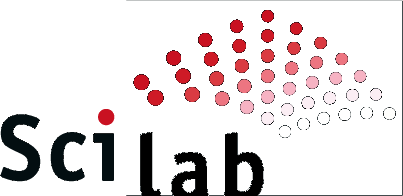
\includegraphics[height=.8cm]{png/logo_scilab}} 
\rotatebox{90}{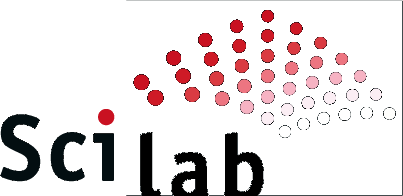
\includegraphics[height=.6cm]{png/logo_scilab}} 
        {\color{violetf}\vrule width 3pt}%
        \hspace{0pt}%must no space.
        \fboxsep=\FrameSep\colorbox{violetc}%
    }%
    \MakeFramed{\hsize #1 \advance\hsize-\width\FrameRestore}%
}%
{\endMakeFramed}%

\newenvironment{pseudo}[1][\hsize]%
{%
    \def\FrameCommand%
    {%
\rotatebox{90}{\textit{\textsf{Pseudo Code}}} 
        {\color{violetf}\vrule width 3pt}%
        \hspace{0pt}%must no space.
        \fboxsep=\FrameSep\colorbox{violetc}%
    }%
    \MakeFramed{\hsize #1 \advance\hsize-\width\FrameRestore}%
}%
{\endMakeFramed}%

\newenvironment{py}[1][\hsize]%
{%
    \def\FrameCommand%
    {%
%\rotatebox{90}{\textit{\textsf{Python}}} 
\rotatebox{90}{
\includegraphics[height=.6cm]{png/logo_python}} 
        {\color{violetf}\vrule width 3pt}%
        \hspace{0pt}%must no space.
        \fboxsep=\FrameSep\colorbox{violetc}%
    }%
    \MakeFramed{\hsize #1 \advance\hsize-\width\FrameRestore}%
}%
{\endMakeFramed}%


\newenvironment{term}[1][\hsize]%
{%
    \def\FrameCommand%
    {%
\rotatebox{90}{\textit{\textsf{Terminal}}} 
        {\color{violetf}\vrule width 3pt}%
        \hspace{0pt}%must no space.
        \fboxsep=\FrameSep\colorbox{violetc}%
    }%
    \MakeFramed{\hsize #1 \advance\hsize-\width\FrameRestore}%
}%
{\endMakeFramed}%



\newenvironment{comp}[1][\hsize]%
{%
    \def\FrameCommand
    {%
\rotatebox{90}{\textit{\textsf{Compétences}}} 
        {\color{bleuf}\vrule width 3pt}%
        \hspace{0pt}%must no space.
        \fboxsep=\FrameSep\colorbox{bleuc}%
    }%
    \MakeFramed{\hsize#1\advance\hsize-\width\FrameRestore}%
}%
{\endMakeFramed}%

\newenvironment{rem}[1][\hsize]%
{%
    \def\FrameCommand
    {%
\rotatebox{90}{\textit{\textsf{Remarque}}} 
        {\color{bleuf}\vrule width 3pt}%
        \hspace{0pt}%must no space.
        \fboxsep=\FrameSep\colorbox{bleuc}%
    }%
    \MakeFramed{\hsize#1\advance\hsize-\width\FrameRestore}%
}%
{\endMakeFramed}%


\newenvironment{savoir}[1][\hsize]%
{%
    \def\FrameCommand
    {%
\rotatebox{90}{\textit{\textsf{Savoir}}} 
        {\color{bleuf}\vrule width 3pt}%
        \hspace{0pt}%must no space.
        \fboxsep=\FrameSep\colorbox{bleuc}%
    }%
    \MakeFramed{\hsize#1\advance\hsize-\width\FrameRestore}%
}%
{\endMakeFramed}%

\newenvironment{Objectif}[1][\hsize]%
{%
    \def\FrameCommand
    {%
\rotatebox{90}{\textit{\textsf{Objectif}}} 
        {\color{bleuf}\vrule width 3pt}%
        \hspace{0pt}%must no space.
        \fboxsep=\FrameSep\colorbox{bleuc}%
    }%
    \MakeFramed{\hsize#1\advance\hsize-\width\FrameRestore}%
}%
{\endMakeFramed}%

\newenvironment{prob}[1][\hsize]%
{%
    \def\FrameCommand%
    {%
\rotatebox{90}{\textit{\textsf{ Problématique}}} 
        {\color{rougef}\vrule width 3pt}%
        \hspace{0pt}%must no space.
        \fboxsep=\FrameSep\colorbox{rougec}%
    }%
    \MakeFramed{\hsize#1\advance\hsize-\width\FrameRestore}%
}%
{\endMakeFramed}%

\newenvironment{obj}[1][\hsize]%
{%
    \def\FrameCommand%
    {%
\rotatebox{90}{\textit{\textsf{Objectifs}}} 
        {\color{rougef}\vrule width 3pt}%
        \hspace{0pt}%must no space.
        \fboxsep=\FrameSep\colorbox{rougec}%
    }%
    \MakeFramed{\hsize#1\advance\hsize-\width\FrameRestore}%
}%
{\endMakeFramed}%

\newenvironment{defi}[1][\hsize]%
{%
    \def\FrameCommand%
    {%
\rotatebox{90}{\textit{\textsf{Définition\\}}} 
        {\color{bleuf}\vrule width 3pt}%
        \hspace{0pt}%must no space.
        \fboxsep=\FrameSep\colorbox{bleuc}%
    }%
    \MakeFramed{\hsize#1\advance\hsize-\width\FrameRestore}%
}%
{\endMakeFramed}%


\newenvironment{demo}[1][\hsize]%
{%
    \def\FrameCommand%
    {%
\rotatebox{90}{\textit{\textsf{Démonstration\\}}} 
        {\color{bleuf}\vrule width 3pt}%
        \hspace{0pt}%must no space.
        \fboxsep=\FrameSep\colorbox{bleuc}%
    }%
    \MakeFramed{\hsize#1\advance\hsize-\width\FrameRestore}%
}%
{\endMakeFramed}%


\newenvironment{hypo}[1][\hsize]%
{%
    \def\FrameCommand%
    {%
\rotatebox{90}{\textit{\textsf{Hypothèse\\}}} 
        {\color{bleuf}\vrule width 3pt}%
        \hspace{0pt}%must no space.
        \fboxsep=\FrameSep\colorbox{bleuc}%
    }%
    \MakeFramed{\hsize#1\advance\hsize-\width\FrameRestore}%
}%
{\endMakeFramed}%


\newenvironment{prop}[1][\hsize]%
{%
    \def\FrameCommand%
    {%
\rotatebox{90}{\textit{\textsf{Propriété\\}}} 
        {\color{bleuf}\vrule width 3pt}%
        \hspace{0pt}%must no space.
        \fboxsep=\FrameSep\colorbox{bleuc}%
    }%
    \MakeFramed{\hsize#1\advance\hsize-\width\FrameRestore}%
}%
{\endMakeFramed}%

\newenvironment{props}[1][\hsize]%
{%
    \def\FrameCommand%
    {%
\rotatebox{90}{\textit{\textsf{Propriétés\\}}} 
        {\color{bleuf}\vrule width 3pt}%
        \hspace{0pt}%must no space.
        \fboxsep=\FrameSep\colorbox{bleuc}%
    }%
    \MakeFramed{\hsize#1\advance\hsize-\width\FrameRestore}%
}%
{\endMakeFramed}%

\newenvironment{exemple}[1][\hsize]%
{%
    \def\FrameCommand%
    {%
\rotatebox{90}{\textit{\textsf{Exemple\\}}} 
        {\color{vertf}\vrule width 3pt}%
        \hspace{0pt}%must no space.
        \fboxsep=\FrameSep\colorbox{vertc}%
    }%
    \MakeFramed{\hsize#1\advance\hsize-\width\FrameRestore}%
}%
{\endMakeFramed}%

\newenvironment{exercice}[1][\hsize]%
{%
    \def\FrameCommand%
    {%
\rotatebox{90}{\textit{\textsf{Exercice\\}}} 
        {\color{vertf}\vrule width 3pt}%
        \hspace{0pt}%must no space.
        \fboxsep=\FrameSep\colorbox{vertc}%
    }%
    \MakeFramed{\hsize#1\advance\hsize-\width\FrameRestore}%
}%
{\endMakeFramed}%

\newenvironment{Support}[1][\hsize]%
{%
    \def\FrameCommand%
    {%
\rotatebox{90}{\textit{\textsf{Support de cours\\}}} 
        {\color{vertf}\vrule width 3pt}%
        \hspace{0pt}%must no space.
        \fboxsep=\FrameSep\colorbox{jaunec}%
    }%
    \MakeFramed{\hsize#1\advance\hsize-\width\FrameRestore}%
}%
{\endMakeFramed}%

\newenvironment{resultat}[1][\hsize]%
{%
    \def\FrameCommand%
    {%
\rotatebox{90}{\textit{\textsf{Résultat\\}}} 
        {\color{rougef}\vrule width 3pt}%
        \hspace{0pt}%must no space.
        \fboxsep=\FrameSep\colorbox{rougec}%
    }%
    \MakeFramed{\hsize#1\advance\hsize-\width\FrameRestore}%
}%
{\endMakeFramed}%

\newenvironment{methode}[1][\hsize]%
{%
    \def\FrameCommand%
    {%
\rotatebox{90}{\textit{\textsf{Méthode\\}}} 
        {\color{rougef}\vrule width 3pt}%
        \hspace{0pt}%must no space.
        \fboxsep=\FrameSep\colorbox{rougec}%
    }%
    \MakeFramed{\hsize#1\advance\hsize-\width\FrameRestore}%
}%
{\endMakeFramed}%

\newenvironment{theo}[1][\hsize]%
{%
    \def\FrameCommand%
    {%
\rotatebox{90}{\textit{\textsf{Théorème\\}}} 
        {\color{rougef}\vrule width 3pt}%
        \hspace{0pt}%must no space.
        \fboxsep=\FrameSep\colorbox{rougec}%
    }%
    \MakeFramed{\hsize#1\advance\hsize-\width\FrameRestore}%
}%
{\endMakeFramed}%

\newenvironment{warn}[1][\hsize]%
{%
    \def\FrameCommand%
    {%
\rotatebox{90}{\textit{\textsf{Attention\\}}} 
        {\color{rougef}\vrule width 3pt}%
        \hspace{0pt}%must no space.
        \fboxsep=\FrameSep\colorbox{rougec}%
    }%
    \MakeFramed{\hsize#1\advance\hsize-\width\FrameRestore}%
}%
{\endMakeFramed}%

%Si le boolen xp est vrai : compilation pour xabi
%Sinon compilation Damien
\newboolean{xp}
\setboolean{xp}{true}

\newboolean{prof}
\setboolean{prof}{true}

\usepackage[%
    pdftitle={Systèmes hydrauliques et pneumatiques},
    pdfauthor={Xavier Pessoles},
    colorlinks=true,
    linkcolor=blue,
    citecolor=magenta]{hyperref}


\def\discipline{Sciences Industrielles de l'Ingénieur}
\def\xxtitre{\ifthenelse{\boolean{xp}}{
CI 1 : Analyse des systèmes pluritechniques et multiphysiques -- Initiation à l'Ingénierie Système}{}}

\def\xxsoustitre{\ifthenelse{\boolean{xp}}{
Chapitre 12 -- Analyse des systèmes hydrauliques et pneumatiques}{
Partie  -- }}

\def\xxauteur{\ifthenelse{\boolean{xp}}{
Xavier \textsc{Pessoles}}{}}

\def\xxpied{\ifthenelse{\boolean{xp}}{
CI 1 : Analyse des systèmes pluritechniques et multiphysiques\\
Ch. 12 : Systèmes hydrauliques et pneumatiques -- Cours}{
\xxtitre}}

\def\xxcathegorie{\ifthenelse{\boolean{xp}}{
2013 -- 2014 \\
Xavier \textsc{Pessoles}}{
Informatique - Cours}}





%---------------------------------------------------------------------------


\begin{document}

\ifthenelse{\boolean{xp}}{
\sloppy
\hyphenpenalty 10000


%------------- En tetes et Pieds de Pages ------------

\pagestyle{fancy}
\renewcommand{\headrulewidth}{0pt}
\fancyhead{}
\fancyhead[L]{%
\noindent\begin{minipage}[c]{2.6cm}%

\includegraphics[width=2cm]{png/logo_ptsi.png}%
\end{minipage}}


\fancyhead[C]{\rule{12cm}{.5pt}}


\fancyhead[R]{%
\noindent\begin{minipage}[c]{3cm}
\begin{flushright}
\footnotesize{\textit{\textsf{\discipline}}}%
\end{flushright}
\end{minipage}
}



\fancyhead[C]{\rule{12cm}{.5pt}}

\renewcommand{\footrulewidth}{0.2pt}

\fancyfoot[C]{\footnotesize{\bfseries \thepage}}
\fancyfoot[L]{%
\begin{minipage}[c]{.2\linewidth}
\noindent\footnotesize{{\xxauteur}}
\end{minipage}
}

\ifthenelse{\boolean{prof}}{%
\fancyfoot[R]{\footnotesize{\xxpied}}}

\begin{center}
 \huge\textsc{\xxtitre}
\end{center}

\begin{center}
 \LARGE\textsc{\xxsoustitre}
\end{center}

\vspace{.5cm}
}{\ifthenelse{\boolean{xp}}{
\usepackage[%
    pdftitle={OS et Environnement de développement},
    pdfauthor={Xavier Pessoles},
    colorlinks=true,
    linkcolor=blue,
    citecolor=magenta]{hyperref}}{
\usepackage[%
    pdftitle={OS et Environnement de développement},
    pdfauthor={Damien Iceta},
    colorlinks=true,
    linkcolor=blue,
    citecolor=magenta]{hyperref}}

\usepackage{pifont}
\usepackage{lastpage}

% \makeatletter \let\ps@plain\ps@empty \makeatother
%% DEBUT DU DOCUMENT
%% =================
\sloppy
\hyphenpenalty 10000

\newcommand{\Pointilles}[1][3]{%
\multido{}{#1}{\makebox[\linewidth]{\dotfill}\\[\parskip]
}}


\colorlet{shadecolor}{orange!15}

\newtheorem{theorem}{Theorem}


\begin{document}


\newboolean{prof}
\setboolean{prof}{true}
%------------- En tetes et Pieds de Pages ------------


\pagestyle{fancy}
%\renewcommand{\headrulewidth}{0}
\renewcommand{\headrulewidth}{0.2pt} %pour mettre le trait en haut

\fancyhead{}
\fancyhead[L]{
\footnotesize{{{\xxtitre}}}%
%\noindent\noindent\begin{minipage}[c]{2.6cm}
%\includegraphics[width=2.5cm]{png/logo.png}%
%\end{minipage}
}

%\fancyhead[C]{\rule{12cm}{.5pt}}  %pour mettre le petit trait en haut


\fancyhead[R]{%
\noindent\begin{minipage}[c]{3cm}
\begin{flushright}
\footnotesize{{{\xxcathegorie}}}%
\end{flushright}
\end{minipage}
}

\renewcommand{\footrulewidth}{0.2pt}

\fancyfoot[C]{\footnotesize{}}
\fancyfoot[L]{%
\begin{minipage}[l]{.2\linewidth}
\noindent\footnotesize{{\xxauteur}}
\end{minipage}
\begin{minipage}[c]{.15\linewidth}
%
\includegraphics[width=2cm]{png/logoCC.png}
\end{minipage}}

\ifthenelse{\boolean{prof}}{%
\fancyfoot[R]{\footnotesize{Page \thepage\   sur  \pageref{LastPage}}}}

\begin{center}
 \huge\textsc{\xxtitre}
\end{center}

\begin{center}
 \LARGE\textsc{\xxsoustitre}
\end{center}

\vspace{.5cm}}

\begin{minipage}[c]{.23\linewidth}
\begin{center}
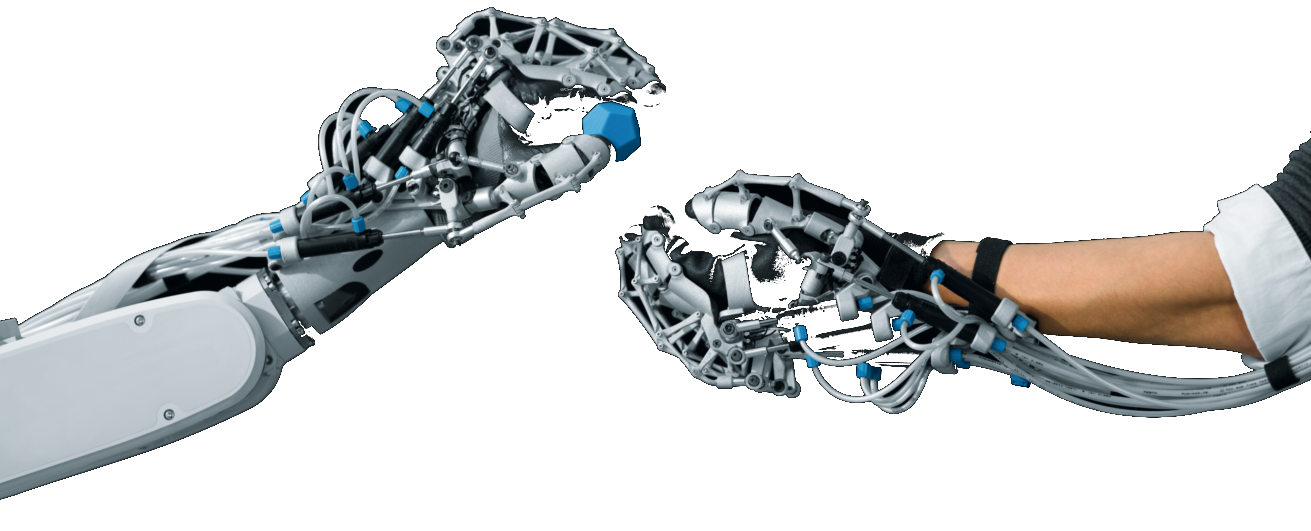
\includegraphics[width=.95\textwidth]{images/ExoHand}

\textit{ExoHand -- Festo \cite{festo}}
\end{center}
\end{minipage} \hfill
\begin{minipage}[c]{.23\linewidth}
\begin{center}
\includegraphics[width=.95\textwidth]{images/caterpillar}

\textit{Pelle hydraulique -- Caterpillar \cite{caterpillar}}
\end{center}
\end{minipage} \hfill
\begin{minipage}[c]{.23\linewidth}
\begin{center}
\includegraphics[width=.95\textwidth]{images/simulateur}

\textit{Simulateur de vol \cite{simulateur}}
\end{center}
\end{minipage} \hfill
\begin{minipage}[c]{.23\linewidth}
\begin{center}
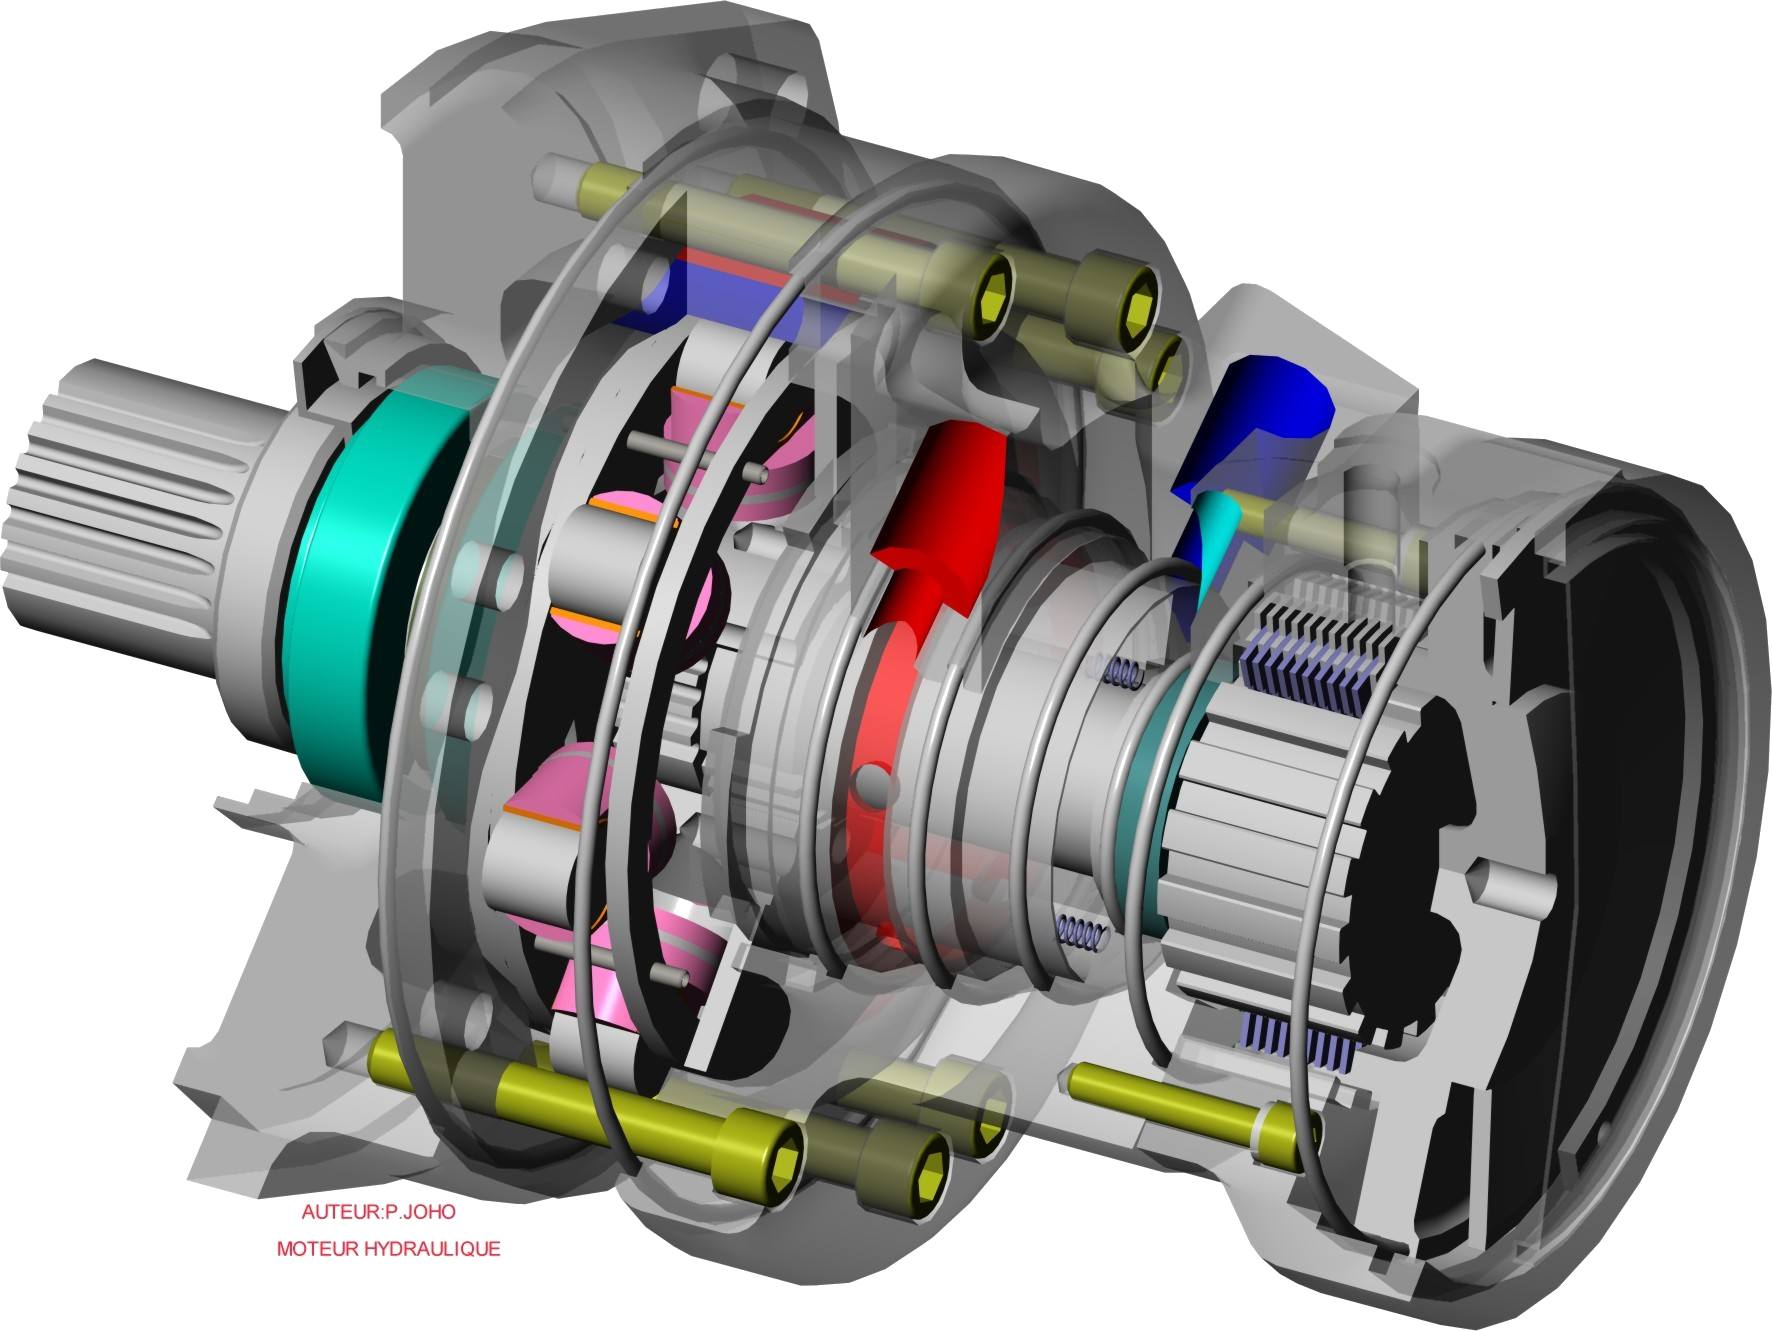
\includegraphics[width=.95\textwidth]{images/MoteurHydraulique}

Moteur hydraulique \cite{mh}
\end{center}
\end{minipage} 

\begin{savoir}
Communiquer : 
\begin{itemize}
\item Com-C2-S1 : Extraire les informations utiles d’un dossier technique;
\item Com-C2-S2 : Effectuer une synthèse des informations disponibles dans un dossier technique;
\item Com-C2-S3 : Vérifier la nature des informations;
\item Com-C2-S4 : Trier les informations selon des critères;
%\item Com-C2-S5 : Distinguer les différents types de documents en fonction de leurs usages;
\item Com-C2-S6 : Lire et décoder un schéma.
\end{itemize}
\end{savoir}


\setlength{\parskip}{0ex plus 0.2ex minus 0ex}
 \renewcommand{\contentsname}{}
 \renewcommand{\baselinestretch}{1}

\tableofcontents

 \renewcommand{\baselinestretch}{1.2}
\setlength{\parskip}{2ex plus 0.5ex minus 0.2ex}



\section{L'énergie pneumatique et hydraulique dans la chaîne fonctionnelle d'un système}

\begin{center}
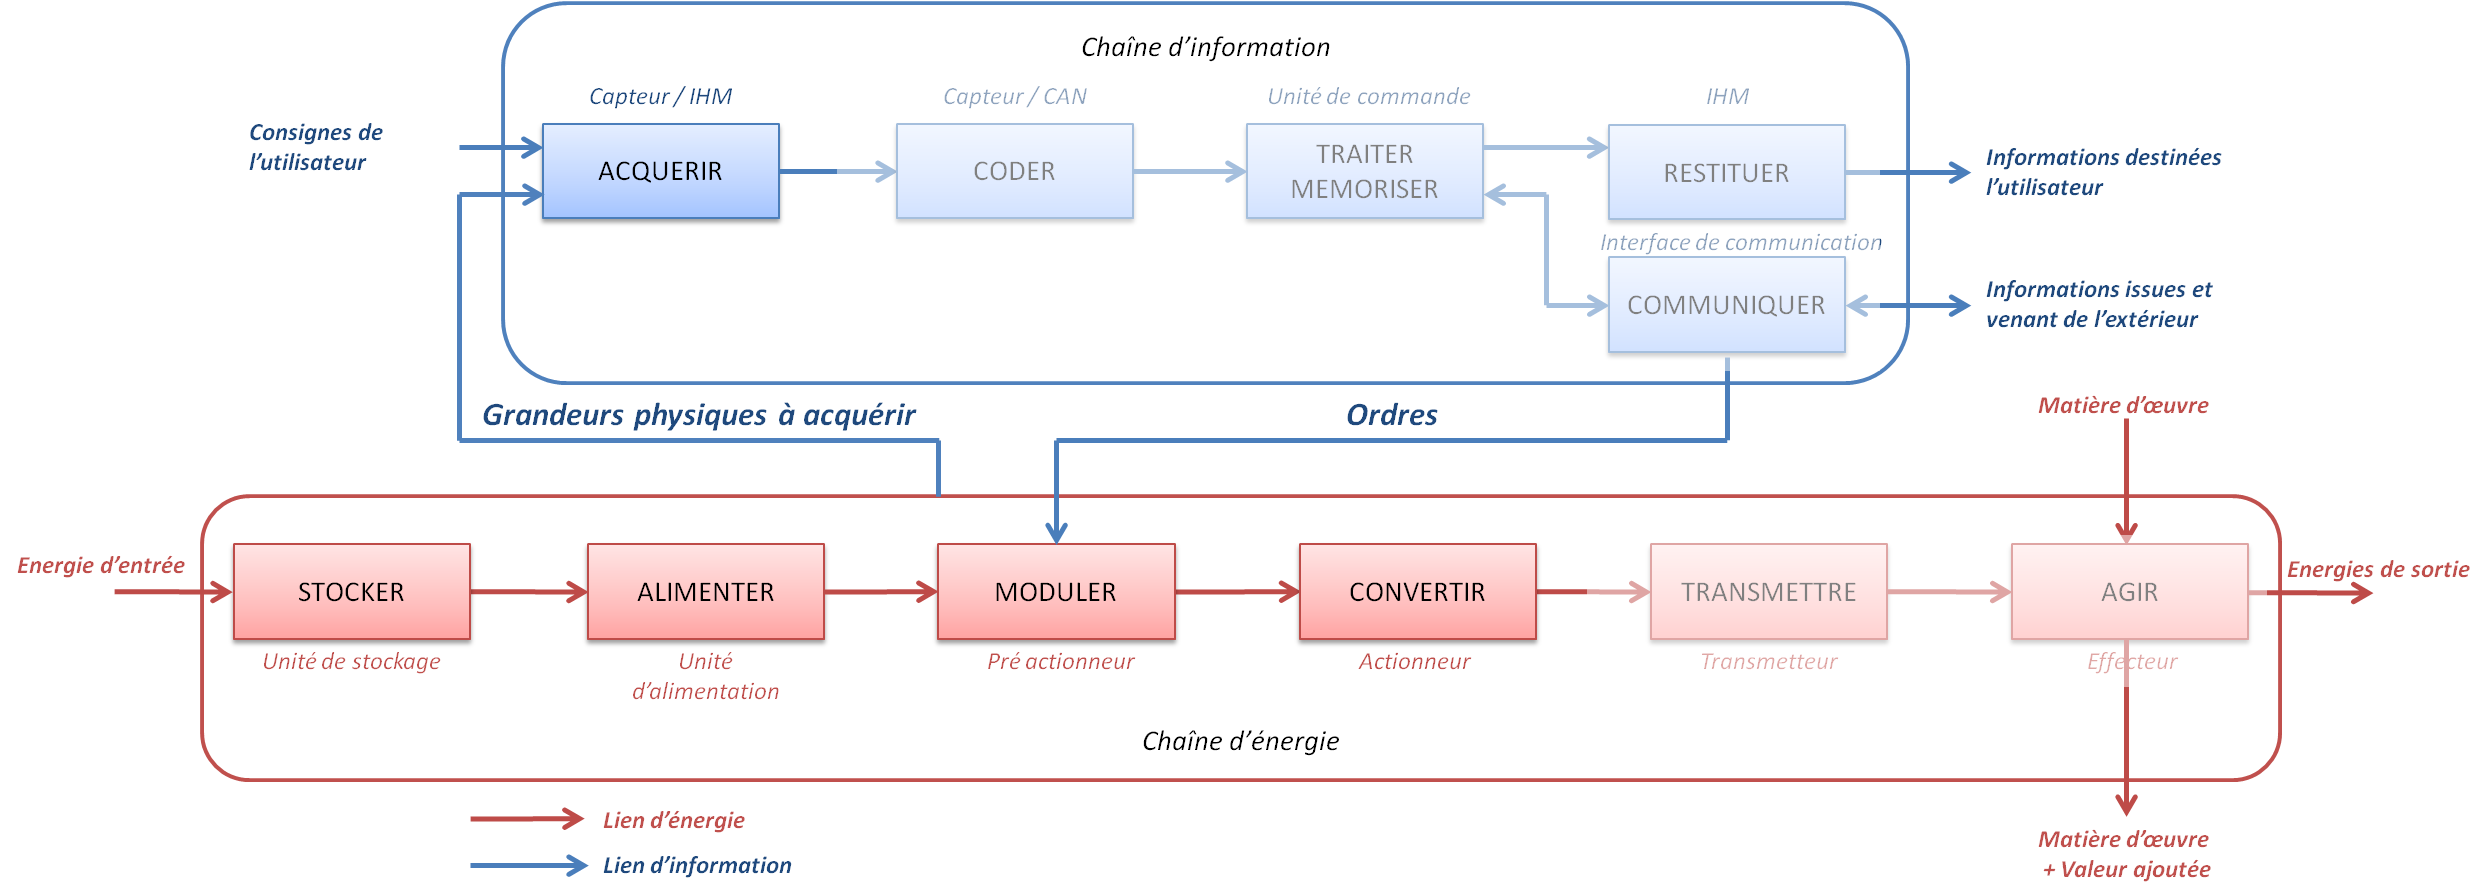
\includegraphics[width=.95\textwidth]{images/chainefonc}
\end{center}

\subsection{Définitions}
\begin{defi}
\textbf{Énergie pneumatique}

Le fluide utilisé est de l’air comprimé.
\end{defi}

\begin{defi}
\textbf{Énergie hydraulique}

Le fluide utilisé est une huile hydraulique minérale ou difficilement inflammable (aqueux ou non).
\end{defi}

L'unité de pression est le Pascal, noté $P$.
\begin{resultat}
$$
1\; bar = 10^5\; Pa \quad 10^6 \; Pa = 1 \; MPa = 1\; N/mm^2
$$
\end{resultat}

Le débit d'un fluide est noté $q$. Il s'exprime en $m^3/s$. 

\begin{resultat}
\textbf{Puissance hydraulique et pneumatique}
La puissance en Watt s'exprime par :
$$ 
\mathcal{P} = qp
$$


\end{resultat}

\subsection{Comparatif}

\begin{center}
\begin{tabular}{|l|p{.35\textwidth}|p{.35\textwidth}|}
\hline
& Avantage & Inconvénients \\
\hline
\hline
Énergie  pneumatique &
\begin{itemize}
\item Production : air disponible partout et en quantité illimitée.
\item Transport aisé dans des conduites bon marché.
\item Matière d’œuvre propre.
\item Composants peu coûteux.
\item Possibilité de vitesses et de cadences élevées.
\end{itemize}
&
\begin{itemize}
\item Source d'énergie exigeant un excellent conditionnement (filtration). Aucune impureté, aucune poussière, etc., ne doit pénétrer dans le système.
\item Difficulté d'obtenir des vitesses régulières du fait de la compressibilité de l'air.
\item Forces développées restent relativement faibles (pression d’utilisation de 3 à 10 bars).
\end{itemize}
 \\
\hline
Énergie hydraulique & 
\begin{itemize}
\item Transmission de forces et de couples élevés.
\item Une grande souplesse d'utilisation dans de nombreux domaines.
\item Une très bonne régulation de la vitesse sur les appareils moteurs, du fait de l'incompressibilité du fluide.
\item Le démarrage en charge des moteurs hydrauliques et des vérins.
\item Une augmentation de la longévité des composants, contrairement aux systèmes pneumatiques, où il est nécessaire d'utiliser un lubrificateur après la filtration de l'air. Les systèmes hydrauliques, du fait de la présence de l'huile, possèdent un excellent moyen de lubrification.
\end{itemize}&
\begin{itemize}
\item Risques d'accident dus à l'utilisation de pressions élevées dans les systèmes 50 < P < 700 bars.
\item Fuites qui entraînent une diminution du rendement.
\item Pertes de charge dues à la circulation de l'huile dans les tuyauteries.
\item Risques d'incendie dus à l'utilisation d'une huile hydraulique minérale inflammable.
\item Matériel coûteux dont la maintenance est onéreuse du fait du prix de revient élevé des composants, du remplacement de l'huile hydraulique et des filtres.
\end{itemize}
\\
\hline
\end{tabular}
\end{center}


\begin{rem}
Les principaux inconvénients de l'air sont résultent de ses propriétés physiques : 
\begin{itemize}
\item sa compressibilité;
\item son échauffement lors de sa compression et son refroidissement en phase de détente;
\item sa masse volumique variable en fonction de la température.
\end{itemize}
En première approximation, ces paramètres sont liés par l'équation des gaz parfaits : $\dfrac{pV}{T} = \text{cte}$ en notant $p$ la pression du gaz, $V$ son volume et $T$ sa température. 

\end{rem}





\section{Stockage et alimentation en énergie}

Pour obtenir de l'énergie pneumatique, on utilise un compresseur. L'énergie hydraulique est obtenue grâce à des pompes. Des exemples de pompes seront données ultérieurement. Les pompes ou les compresseurs sont actionnés par un moteur électrique ou thermique. Dans les systèmes pneumatiques, la circulation d'air se fait généralement en circuit ouvert. Dans le cas des systèmes hydrauliques, le fluide est en circuit fermé. Cela impose des conditions sur les constituants des réseaux. 

\begin{minipage}[b]{.3\textwidth}
\begin{center}
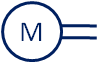
\includegraphics[width=.3\textwidth]{images/Symb_Moteur}

\textit{Symboles d'un moteur}
\end{center}
\end{minipage}\hfill
\begin{minipage}[b]{.3\textwidth}
\begin{center}
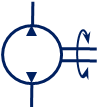
\includegraphics[width=.3\textwidth]{images/Symb_Pompe2}

\textit{Symboles d'une pompe à deux sens de rotation et deux sens de flux}
\end{center}
\end{minipage}\hfill
\begin{minipage}[b]{.3\textwidth}
\begin{center}
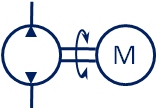
\includegraphics[width=.3\textwidth]{images/Symb_MotoPompe}

\textit{Symboles d'une groupe moteur + pompe}
\end{center}
\end{minipage}

\subsection{Systèmes de stockage}
Dans le cas de l'huile, elle peut être stockée à pression atmosphérique dans un réservoir (appelé aussi <<bâche>>) ou dans un réservoir haute pression. 
Les compresseurs pneumatiques sont souvent reliés à une cuve qui garde l'air sous pression. 


\begin{minipage}[c]{.3\textwidth}
\begin{center}
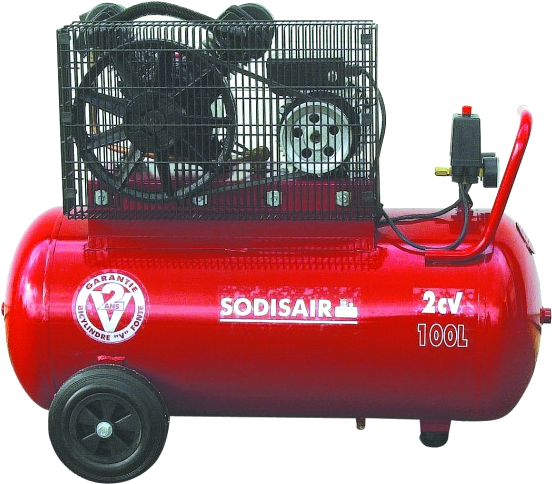
\includegraphics[width=.8\textwidth]{images/Compresseur}

\textit{Compresseur 100L -- 10 bars \cite{compresseur}}
\end{center}
\end{minipage} \hfill
\begin{minipage}[c]{.3\textwidth}
\begin{center}
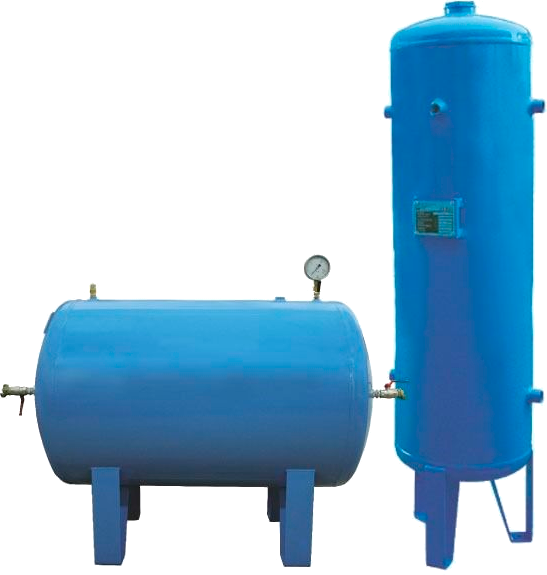
\includegraphics[width=.8\textwidth]{images/reservoir}

\textit{Réservoir de 50 à 25 000 L\cite{reservoir}}
\end{center}
\end{minipage} \hfill
\begin{minipage}[c]{.3\textwidth}
\begin{center}

\includegraphics[width=.3\textwidth]{images/Symb_Reservoir}
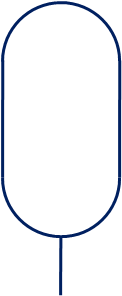
\includegraphics[width=.2\textwidth]{images/Symb_Accumulateur}

\textit{Symboles du réservoir et de l'accumulateur}
\end{center}
\end{minipage}

\subsection{Systèmes de conditionnement}


\begin{minipage}[c]{.55\textwidth}
Il est nécessaire de conditionner le fluide avant de la faire circuler dans le circuit. Dans le cas de l'énergie pneumatique, il est indispensable de s'assurer de la pureté de l'air ainsi que d'un faible taux d'humidité. Pour cela on utilise d'une part des filtres permettant de filtrer l'air entrant dans le réseau en amont et en aval du compresseur. Il est aussi nécessaire d'utiliser d'un refroidisseur-assécheur permettant de réduire le taux d'humidité. 

Dans le cas d'un système hydraulique, le fluide est filtrée afin d'éliminer les impuretés.
\end{minipage} \hfill
\begin{minipage}[c]{.4\textwidth}
\begin{center}
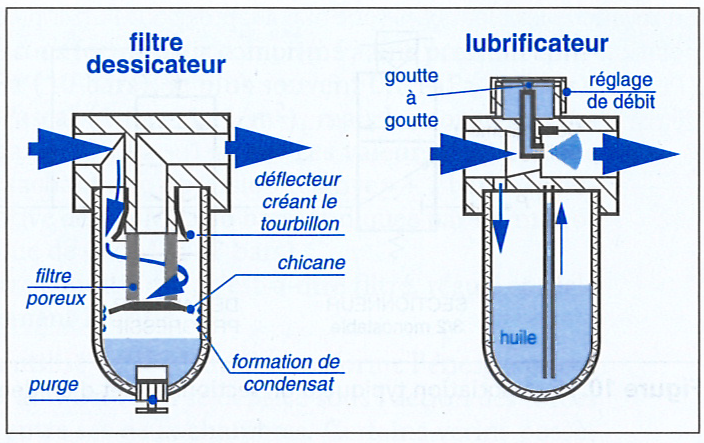
\includegraphics[width=.95\textwidth]{images/fig8}
\end{center}
\end{minipage}



\begin{minipage}[c]{.3\textwidth}
\begin{center}
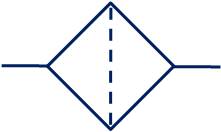
\includegraphics[width=.3\textwidth]{images/Symb_Filtre}

\textit{Symboles d'un filtre}
\end{center}
\end{minipage} \hfill
\begin{minipage}[c]{.3\textwidth}
\begin{center}
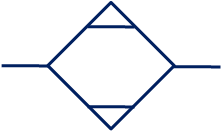
\includegraphics[width=.3\textwidth]{images/Symb_Deshydrateur}

\textit{Symboles d'un déshydrateur}
\end{center}
\end{minipage} \hfill
\begin{minipage}[c]{.3\textwidth}
\begin{center}
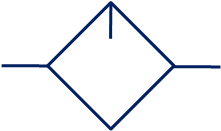
\includegraphics[width=.3\textwidth]{images/Symb_Lubrificateur}

\textit{Symboles d'un lubrificateur}
\end{center}
\end{minipage} 



\subsection{Systèmes de sécurité}


\begin{minipage}[c]{.62\textwidth}
Afin de maîtriser la pression dans les conduites, on peut avoir recours à des manomètres afin d'avoir une informations sur la pression. Les régulateurs de pression permettent quant à eux d'évacuer l'air du système lorsque la pression est trop grande. Les limiteurs de débit permettent de maitriser le débit de fluide.

Les systèmes de clapet anti-retour permettent d'imposer le sens de circulation d'un fluide. 

\end{minipage} \hfill
\begin{minipage}[c]{.35\textwidth}
\begin{center}
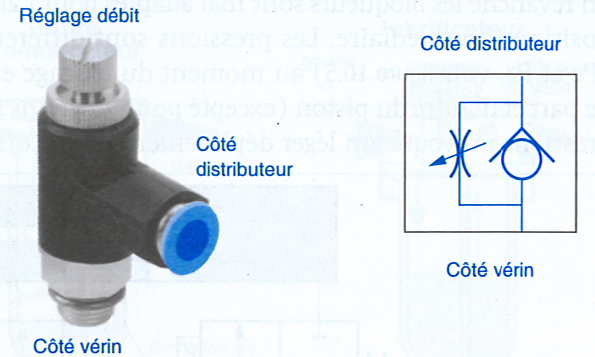
\includegraphics[width=.95\textwidth]{images/fig5}

\textit{Régulateur de débit}
\end{center}
\end{minipage}


\subsection{Exemples}

\begin{minipage}[c]{.47\textwidth}
\begin{center}
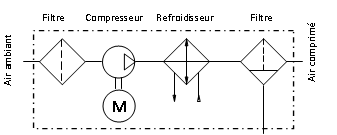
\includegraphics[width=.95\textwidth]{images/Fig_01_Compresseur}

\textit{Schéma de compresseur intégré}
\end{center}
\end{minipage} \hfill
\begin{minipage}[c]{.5\textwidth}
\begin{center}
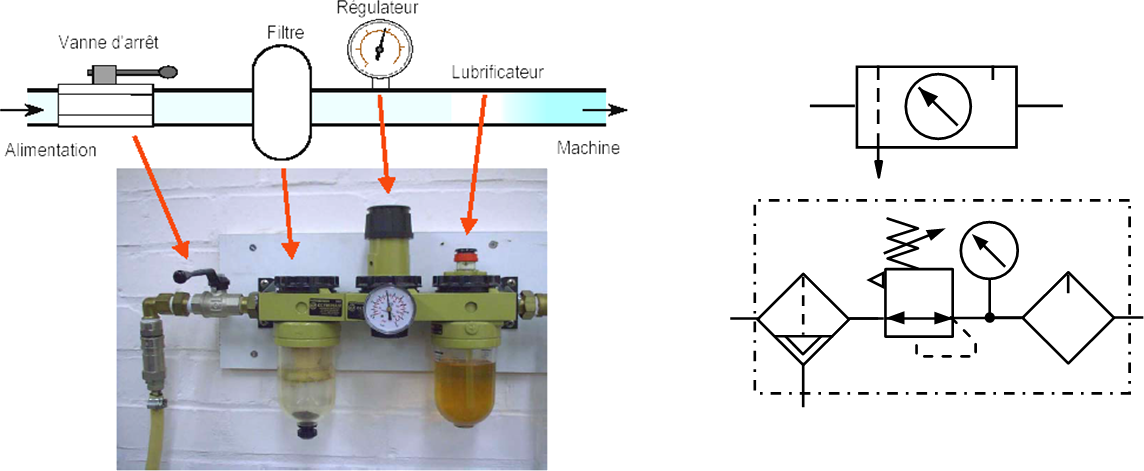
\includegraphics[width=\textwidth]{images/Fig_02_FRL}

\textit{Unité Filtre -- mano-Régulateur -- Lubrificateur}
\end{center}
\end{minipage} 


\section{Convertisseurs d'énergie}
\subsection{Les vérins}
\subsubsection{Constituants d'un vérin}



\begin{minipage}[c]{.47\textwidth}
Un vérin est un actionneur utilisant de l'énergie pneumatique pour produire une énergie mécanique lors d'un déplacement linéaire ou rotatif limité à sa course. Le vérin permet de convertir de l'énergie pneumatique (ou hydraulique) en énergie mécanique.

\begin{center}
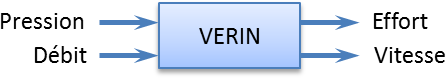
\includegraphics[width=6cm]{images/fig1}
\end{center}
\end{minipage} \hfill
\begin{minipage}[c]{.5\textwidth}
\begin{center}
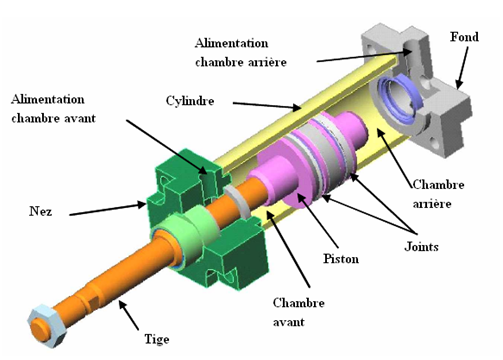
\includegraphics[width=\textwidth]{images/Fig_03_Verin}
\end{center}
\end{minipage}

Dans les deux cas le produit des deux valeurs donne une puissance, la puissance $P\cdot Q$ pneumatique étant convertie en puissance $F\cdot V$ mécanique. Il est à noter que le rendement de ces actionneurs est mauvais ($\eta =0,5$ environ) : une grande partie de l'énergie pneumatique est perdue sous forme d'énergie calorifique et lors de la mise à l'échappement de l'air comprimé. En prenant en compte le rendement du compresseur ($\eta =0,4$), on obtient un rendement global très faible pour la chaîne d'action pneumatique ($\eta =0,2$).

\subsubsection{Fonctionnement d'un vérin pneumatique}

\begin{minipage}[c]{.47\textwidth}
Considérons le vérin représenté par un distributeur à deux positions. On note $Pa$, la pression dans la chambre coté admission, $Pe$, la pression dans la chambre coté échappement (parfois appelée "contre pression d'échappement") et $Pu$, la pression d'utilisation fournie par le secteur pneumatique. 


Au moment précis où le distributeur vient de commuter sous l'action de la commande $v+$, la chambre arrière est brusquement reliée à la pression d'utilisation et simultanément la chambre avant est mise à la pression atmosphérique.

Le déplacement de l'ensemble tige et piston s'effectue en trois phases.

\end{minipage} \hfill
\begin{minipage}[c]{.5\textwidth}
\begin{center}
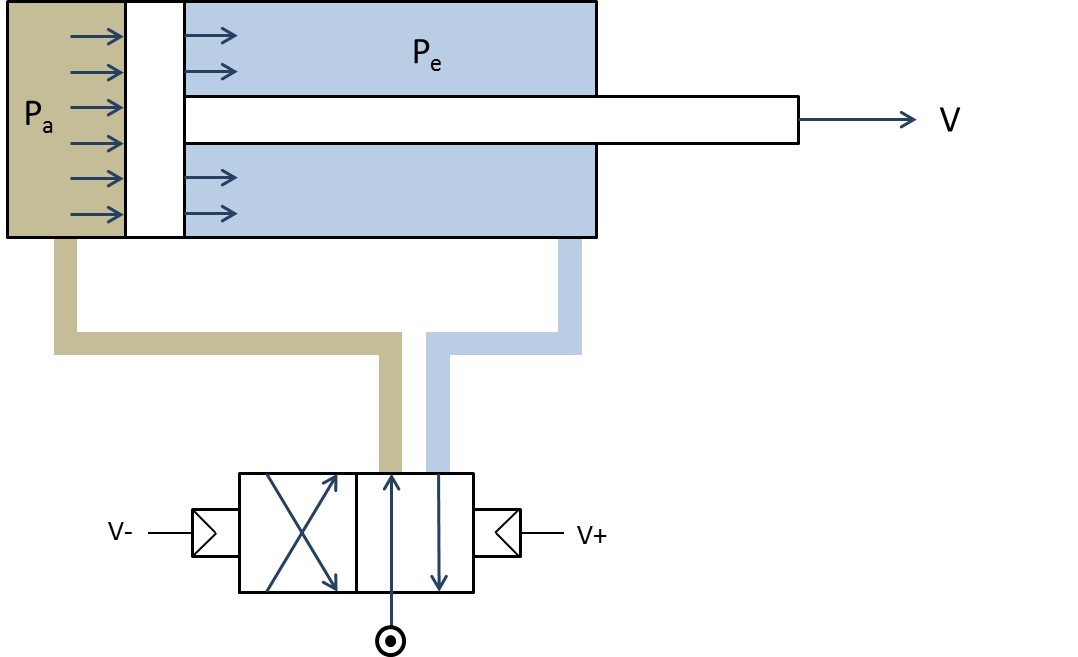
\includegraphics[width=.9\textwidth]{images/fig2}
\end{center}
\end{minipage}


\textbf{Phase 1 : démarrage, de $t=0$ à $t_1$ :} 

La pression $Pa$ augmente progressivement pendant que la pression $Pe$ diminue. Pendant cette phase, de courte durée, le piston est immobile.

\textbf{Phase 2 : déplacement, de $t_1$ à $t_2$} 

Dès que la différence des pressions $Pa-ë$ est suffisante pour vaincre les efforts résistants, le piston se déplace. Pendant cette phase, la pression diminue dans la chambre à l'admission, car le débit d'air ne peut pas compenser l'augmentation du volume de la chambre, et dans la chambre d'échappement pour les raisons inverses. La vitesse du vérin augmente. 

\textbf{Phase 3 : arrêt, de $t_2$ à après }

Lorsque le piston arrive en butée avant du vérin il se produit un arrêt brutal, la vitesse chute quasi instantanément. Les pressions s'équilibrent assez rapidement pour atteindre la pression d'utilisation dans la chambre à l'admission et la pression atmosphérique dans la chambre à l'échappement. 

\paragraph{Système d'amortissement intégré}
Ce qui précède permet de constater que, dans le cas où le vérin travaille sur la totalité de sa course, un choc important a lieu en fin de course. En utilisation l'ensemble des éléments mobile liés à sa tige. Pour ce faire les vérins sont dotés de dispositifs d'amortissement de deux types : 
\begin{itemize}
\item amortissement élastique intégré, il s'agit de bagues élastomères qui ne peuvent absorber qu'une énergie faible;
\item amortissement pneumatique intégré, ces derniers, plus efficaces, sont réglables par vis. 
\end{itemize}

Le principe d'un amortisseur intégré est le suivant : tant que le piston est éloigné de la zone d'amortissement, l'échappement s'effectue normalement. Dès que le piston rentre dans la zone d'amortissement, il vient obturer le cylindre d'échappement : l'air doit alors passer par la restriction réglable ce qui augmente le contre pression $Pe$ et diminue la vitesse. 


\begin{center}
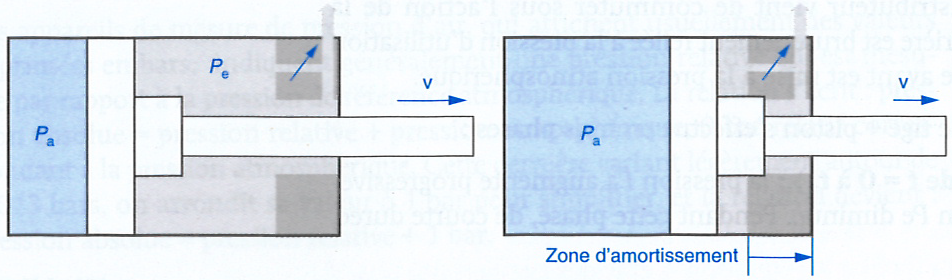
\includegraphics[width=12cm]{images/fig3}
\end{center}

\paragraph{Efforts développés par un vérin}
Pour les raisons déjà évoquées de complexité de modélisation du comportement de l'air, les constructeurs ne fournissent pas de courbes caractéristiques de fonctionnement pour ce type d'actionneur, contrairement aux moteurs électriques ou aux vérins hydrauliques. Afin de pouvoir mener des calculs, on introduit les hypothèses simplificatrices suivantes. 

\paragraph{Effort statique (ou théorique)}
Il correspond à l'effort développé par le vérin en butée. En considérant que la liaison entre cylindre et piston + tige est parfaite, que la pression motrice $Pa$ est constante et égale à la pression d'utilisation $Pa=Pu=P$ et que la contre pression d'échappement $Pe$ est nulle, l'effort statique développé par un vérin est :
$$
F_s=P\cdot S_u
$$
On note $P$ la pression d'utilisation, $S_u$, surface utile du piston. Dans le cas des vérins à tige, l'effort statique en rentrée $F_{sr}$ est différent de celui en sortie $F_{ss}$, les surfaces utiles étant différentes. 

En posant $D$ le diamètre du piston et $d$ le diamètre de la tige, on obtient : 
$$
F_{ss}=P\dfrac{\pi D^2}{4} \quad \text{et} \quad F_{sr}=P\dfrac{\pi \left(D^2-d^2\right)}{4}
$$


\subsubsection{Vérin simple effet}

Ce vérin ne peut développer un effort que dans un seul sens.
La course de rentrée s’effectue grâce à un ressort de rappel incorporé entre le piston et le flasque avant. Il ne possède qu’une seule entrée d’air.

\begin{center}
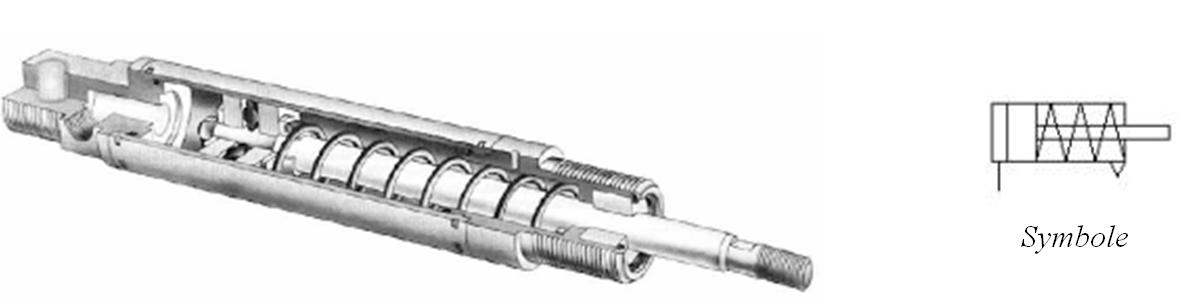
\includegraphics[width=12cm]{images/Fig_04_VerinSE}
\end{center}

\subsubsection{Vérin double effets}
Ce type de vérin peut fournir un travail en tirant et en poussant.

\begin{center}
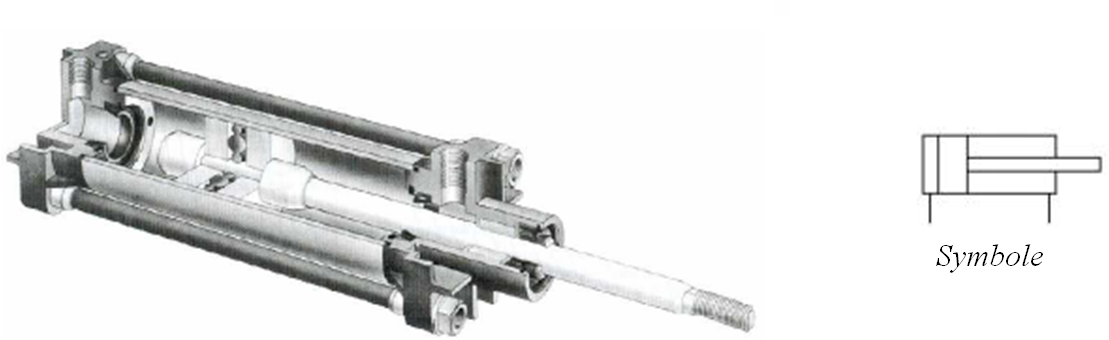
\includegraphics[width=12cm]{images/Fig_05_VerinDE}
\end{center}

\subsubsection{Vérin rotatif}

Le mouvement de translation d’un ensemble tige / piston est transformé en rotation.

\begin{center}
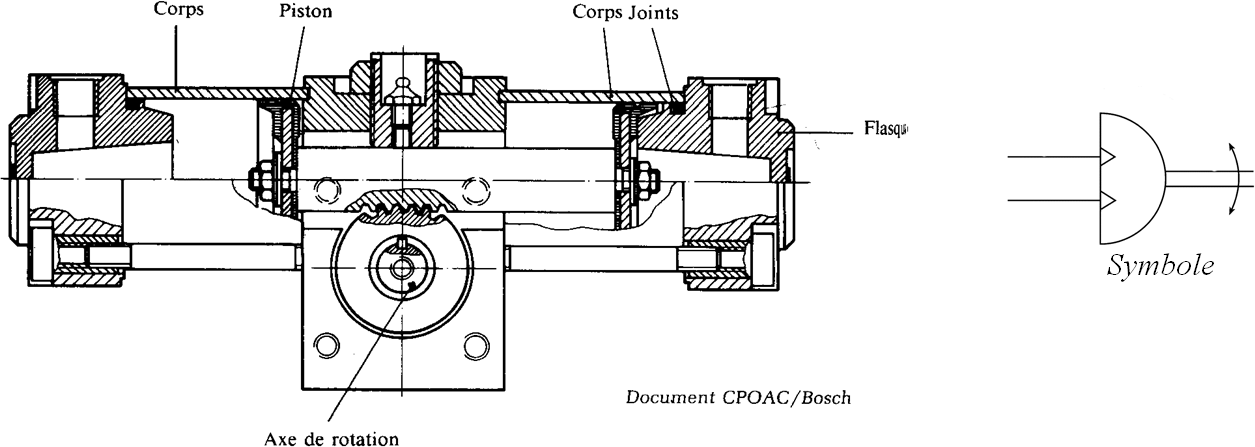
\includegraphics[width=12cm]{images/Fig_06_VerinRot}
\end{center}


\subsection{Moteurs et pompes}

\section{Distributeurs (\textit{modulateurs}) d'énergie}
\subsection{Présentation}



\begin{minipage}[c]{.6\textwidth}
Les distributeurs sont les préactionneurs des vérins pneumatiques et hydrauliques.
Ils servent d’<<aiguillages>> en dirigeant le fluide dans certaines directions.
Les plus utilisés sont les distributeurs à tiroir.

\end{minipage} \hfill
\begin{minipage}[c]{.37\textwidth}
\begin{center}
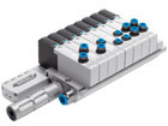
\includegraphics[width=.75\textwidth]{images/distributeur_festo}

\textit{Vérin double effet et distributeur 5/2 monostable à commande manuelle par bouton}
\end{center}
\end{minipage}


\begin{minipage}[c]{.47\textwidth}
\begin{center}
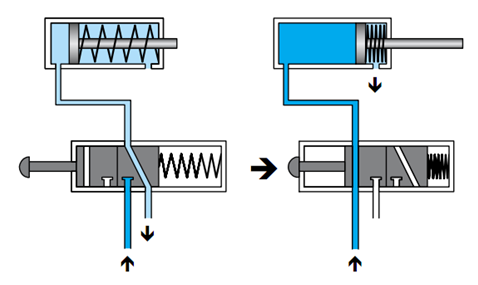
\includegraphics[width=.9\textwidth]{images/Fig_07}

\textit{Vérin simple effet et distributeur 3/2 monostable NF à commande manuelle par bouton}
\end{center}
\end{minipage} \hfill
\begin{minipage}[c]{.47\textwidth}
\begin{center}
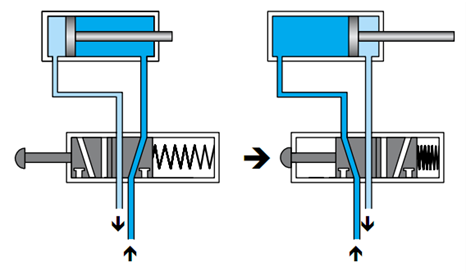
\includegraphics[width=.9\textwidth]{images/Fig_08}

\textit{Vérin double effet et distributeur 5/2 monostable à commande manuelle par bouton}
\end{center}
\end{minipage}


\begin{center}
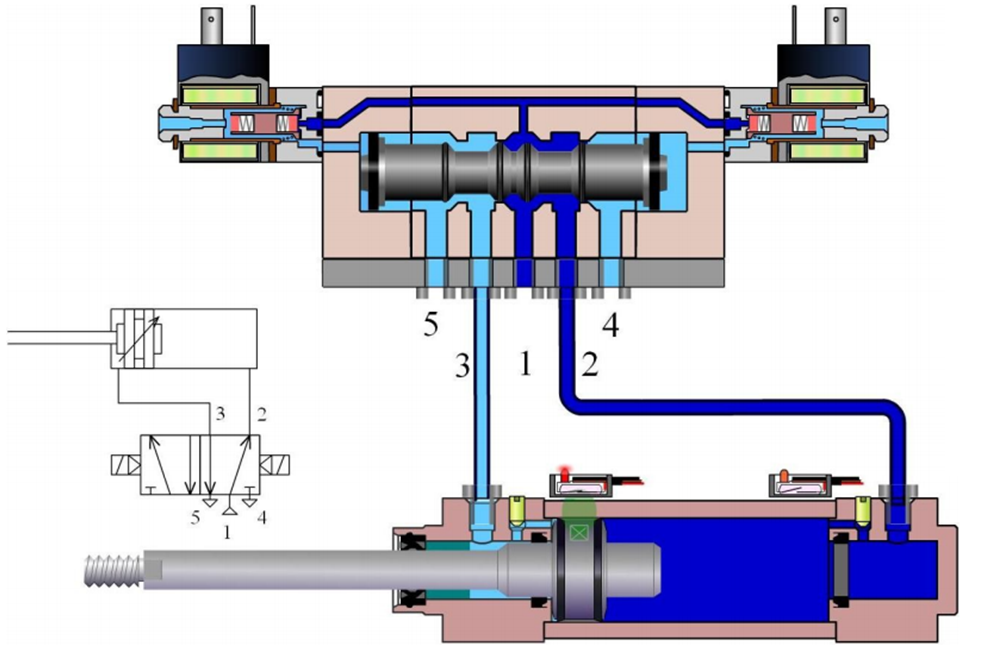
\includegraphics[width=.9\textwidth]{images/Fig_09}

\textit{Vérin double effet à amortissement réglable et distributeur 5/2 bistable à commande électropneumatique}
\end{center}

\subsection{Désignation des distributeurs}
Lors de l'élaboration des schémas, il n'est pas possible de représenter le distributeur, ainsi que les autres composants, sous leurs formes commerciales. De ce fait, l'utilisation de symboles normalisés simplifie la lecture et la compréhension des systèmes. Cette représentation utilise la symbolisation par cases.
Un distributeur se représente sur les côtés droit et/ou gauche (comme dans la réalité) par des pilotages. Ils permettent au tiroir de se déplacer afin de mettre en communication les différents orifices.

\begin{center}
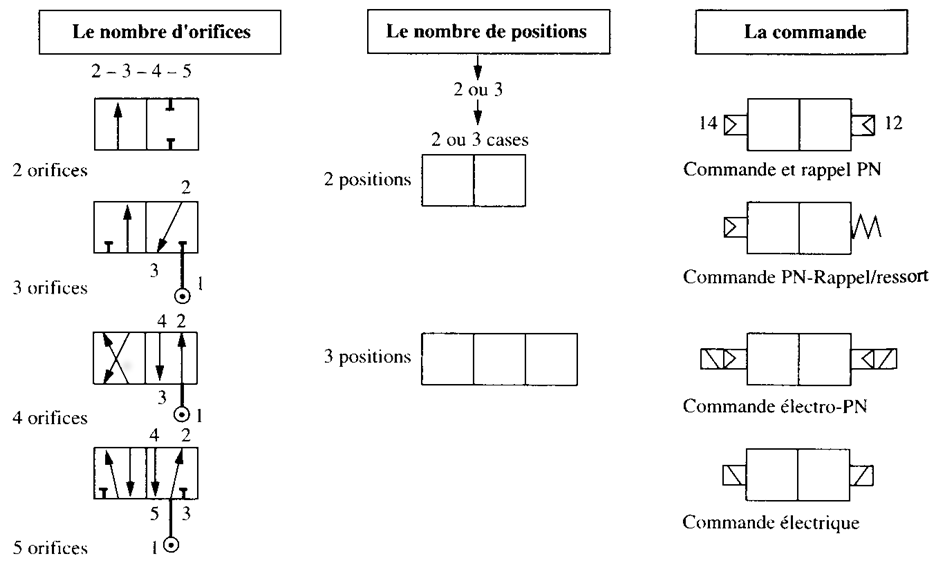
\includegraphics[width=.9\textwidth]{images/Fig_10_distri}
\end{center}

\begin{center}
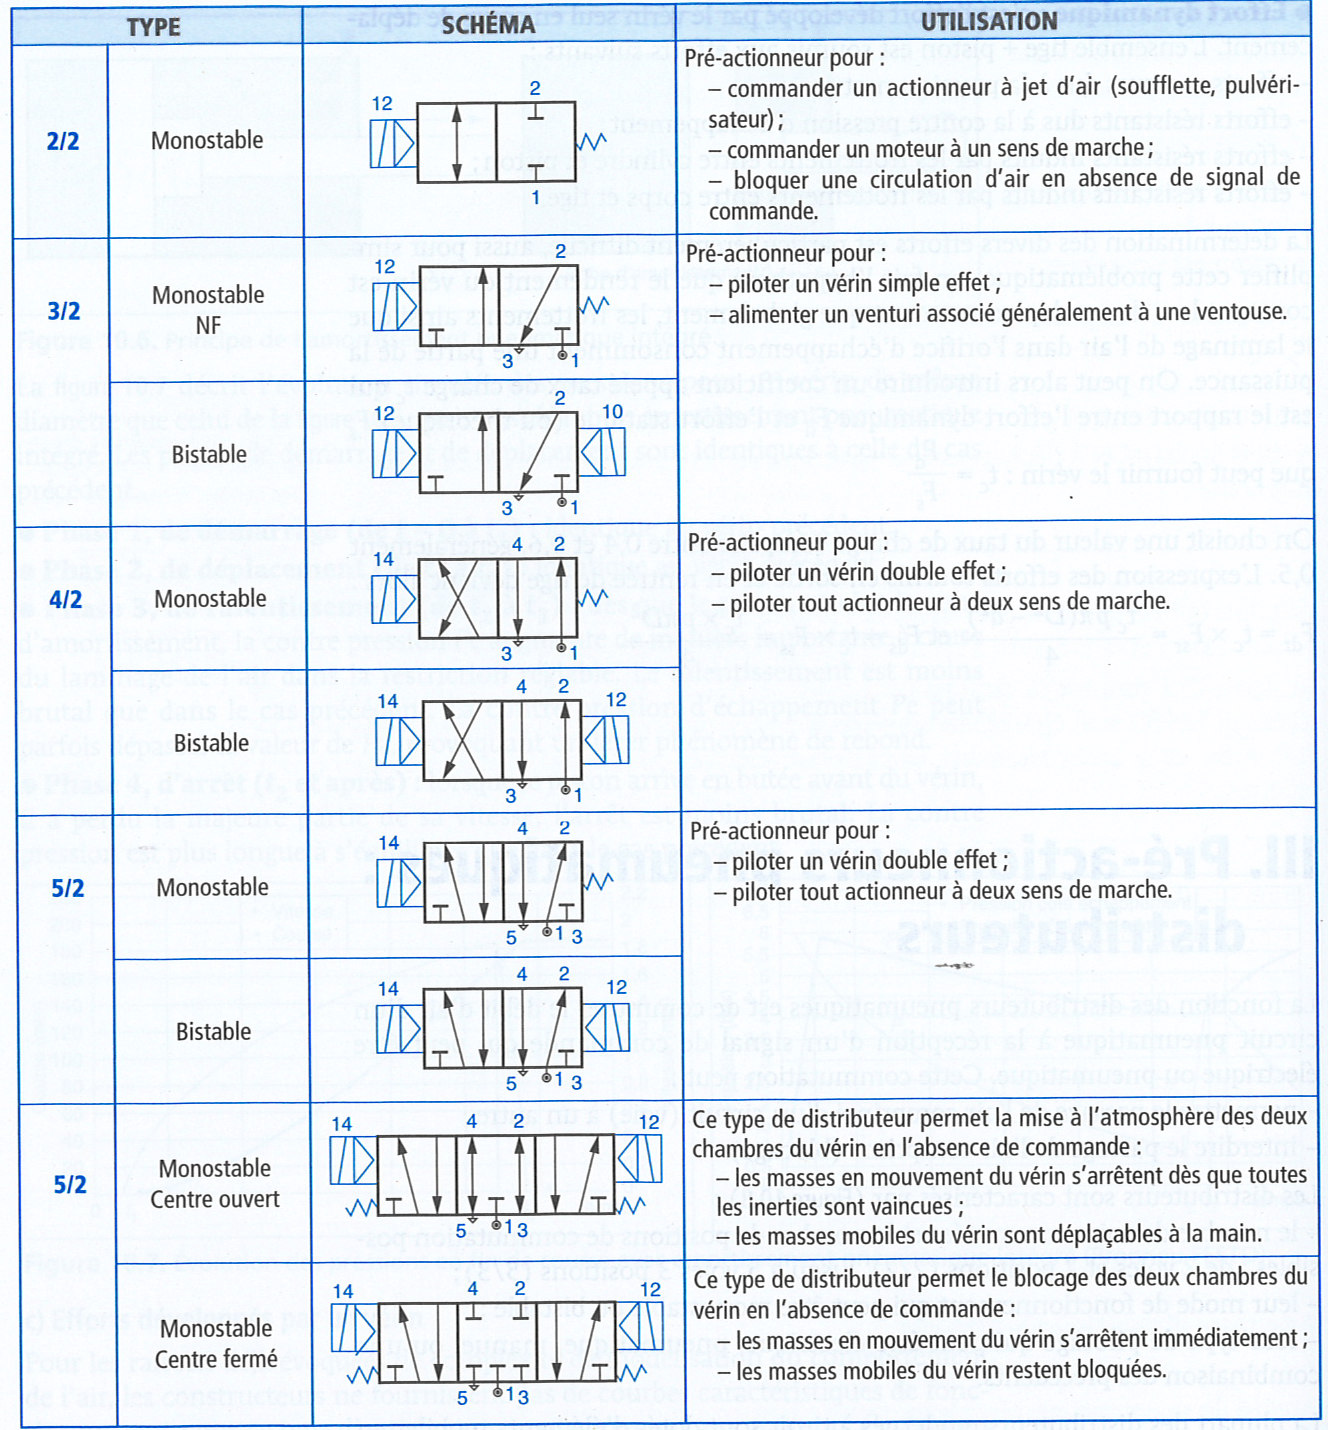
\includegraphics[width=.9\textwidth]{images/fig4}
\end{center}



\section{Actionneurs pneumatiques}
\subsection{Ventouses}
\section{Systèmes de mesure}
\newpage
\section{Récapitulatifs}
\begin{center}
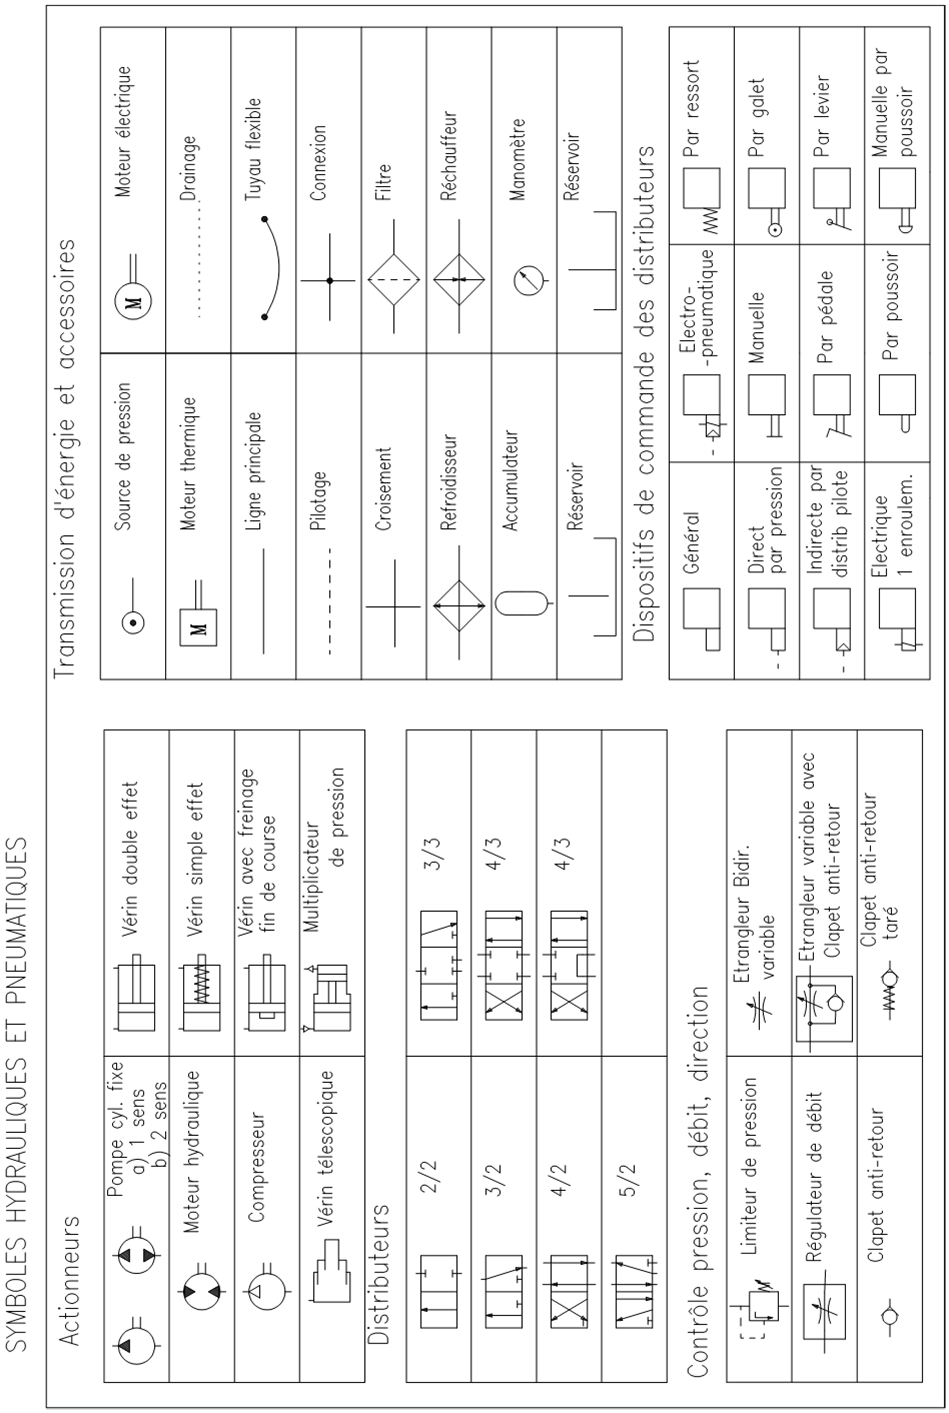
\includegraphics[width=.75\textwidth]{images/recap}
\end{center}

\begin{thebibliography}{2}
\bibitem{festo}{\url{http://www.festo.com}.}
\bibitem{caterpillar}{Caterpillar -- Pelles hydrauliques 374 D L\url{http://s7d2.scene7.com/is/content/Caterpillar/C633539}.}
\bibitem{simulateur}{\url{http://www.defense.gouv.fr/}.}
\bibitem{mh}{\url{http://joho.p.free.fr/}.}
\bibitem{compresseur}{\url{http://www.espaceoutillage.com/}.}
\bibitem{reservoir}{\url{http://www.directindustry.fr/}.}
\bibitem{pb}{\textit{Patrick Beynet}, Fonctions du produit -- Technologie pneumatique – hydraulique pour les systèmes automatisés de production. Lycée Rouvière Toulon.}
\bibitem{perrin}{\textit{J. Perrin, F. Binet, J.-J. Dumery, C. Merlaud, J.-P. Trichard}, Automatique et Informatique Industrielle -- Bases théoriques, méthodologiques et techniques, Éditions Nathan Technique, 2004.}
\end{thebibliography}
\end{document}


